\section{Basic knowledge}
This chapter explains the basics of quantum circuits, quantum gates, and beam searches.
\subsection{Quantum circuits}
Quantum circuits are quantum computing\cite{deutsch1985quantum}
expressed using quantum gates and quantum bits.
Quantum bits and quantum gates are equivalent to bits and logic gates in conventional computers.
Quantum gates have inputs and outputs, just like conventional logic gates.
The desired calculation can be achieved by combining multiple quantum gates.
Quantum circuits have a different property from logic circuits in that they must always be reversible.
In other words, quantum circuits must be able to uniquely determine the input from the output.
\par
\begin{figure}[tbp]
\centering
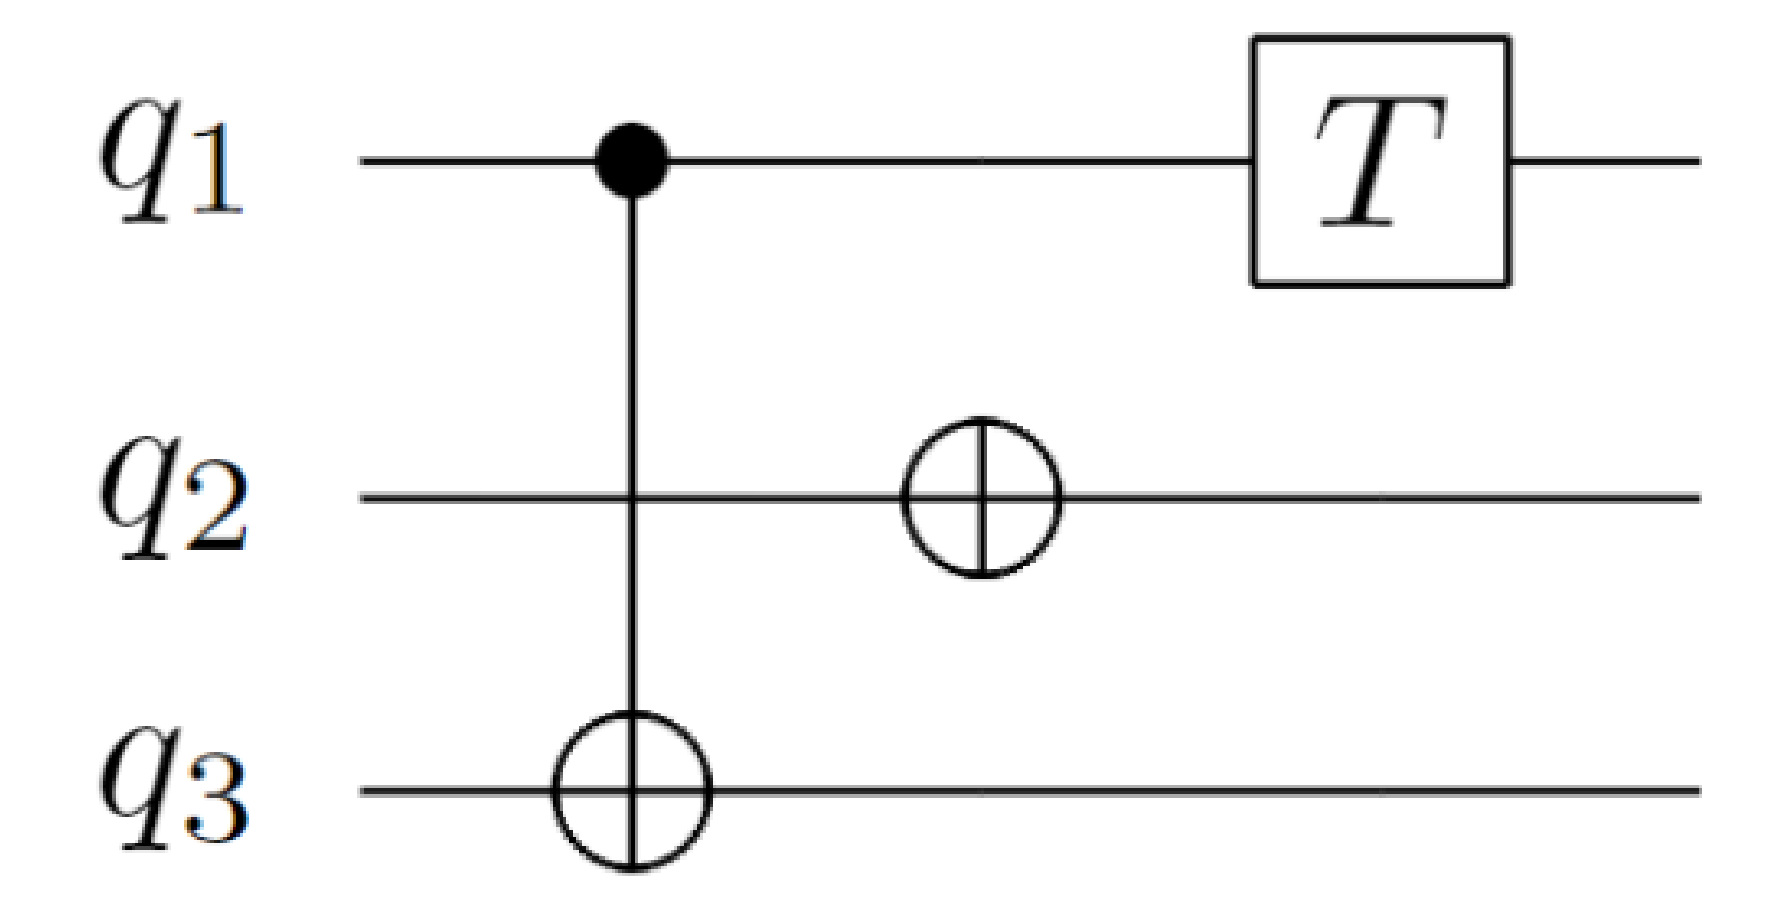
\includegraphics[width=7cm]{img/qcircuit.pdf}
\caption{Example of a quantum circuit}
\label{qcircuit}
\end{figure}
An example of a quantum circuit is shown in Figure ~\ref{qcircuit}.
The horizontal lines labeled $q_{1}$, $q_{2}$, and $q_{3}$ in Figure~\ref{qcircuit}
represent quantum bits.
Quantum gates are illustrated with symbols corresponding to each gate as in Figure~\ref{qcircuit}.
In a quantum circuit, the left side is the input and the right side is the output.
Therefore, quantum gates are executed in order from the left gate.
\subsection{Quantum Gates}
Quantum gates have the function of changing the quantum state of a quantum bit.
A quantum gate has a quantum bit as input, and is composed of a control bit and a target bit.
Some quantum gates do not have a control bit.
The control bit is a quantum bit that determines whether the quantum gate acts on the target bit.
When the value of the control bit is 1, the quantum gate acts on the target bit.
On the other hand, the target bit is a quantum bit whose state is changed by the result of the quantum gate operation when the condition of the control bit is satisfied.
\par
There is a group of quantum gates called Clifford+T\cite{zhou2000methodology}
which consists of $NOT, CNOT, H, T, and T^{\dagger}$ gates.
\gout{A fault-tolerant quantum computing framework that performs the desired calculation while correcting errors.}
To perform an operation, quantum gates must be decomposed into this Clifford+T gate group\cite{boykin2000new}.
\par
\bout{The operation that reverses the operation performed by a quantum gate on a quantum bit is called an inverse transformation.
A quantum gate that performs an inverse transformation can be expressed by adding $\dag$.
For example, the inverse transformation of a $T$ gate is a $T^{\dag}$ gate.
By applying a $T^{\dag}$ gate after applying a $T$ gate,
it is possible to return to the state before the $T$ gate was applied. }
\subsection{NOT gate}
The NOT gate has the same function as the NOT gate in a conventional computer. An example of a NOT gate is shown in
Figure~\ref{not_gate}. A NOT gate is a gate that consists of only one quantum bit, a target bit.
If the value of the target bit is $0$, the NOT gate outputs $1$, and if it is $1$, it outputs $0$.
\begin{figure}[tbp]
\centering
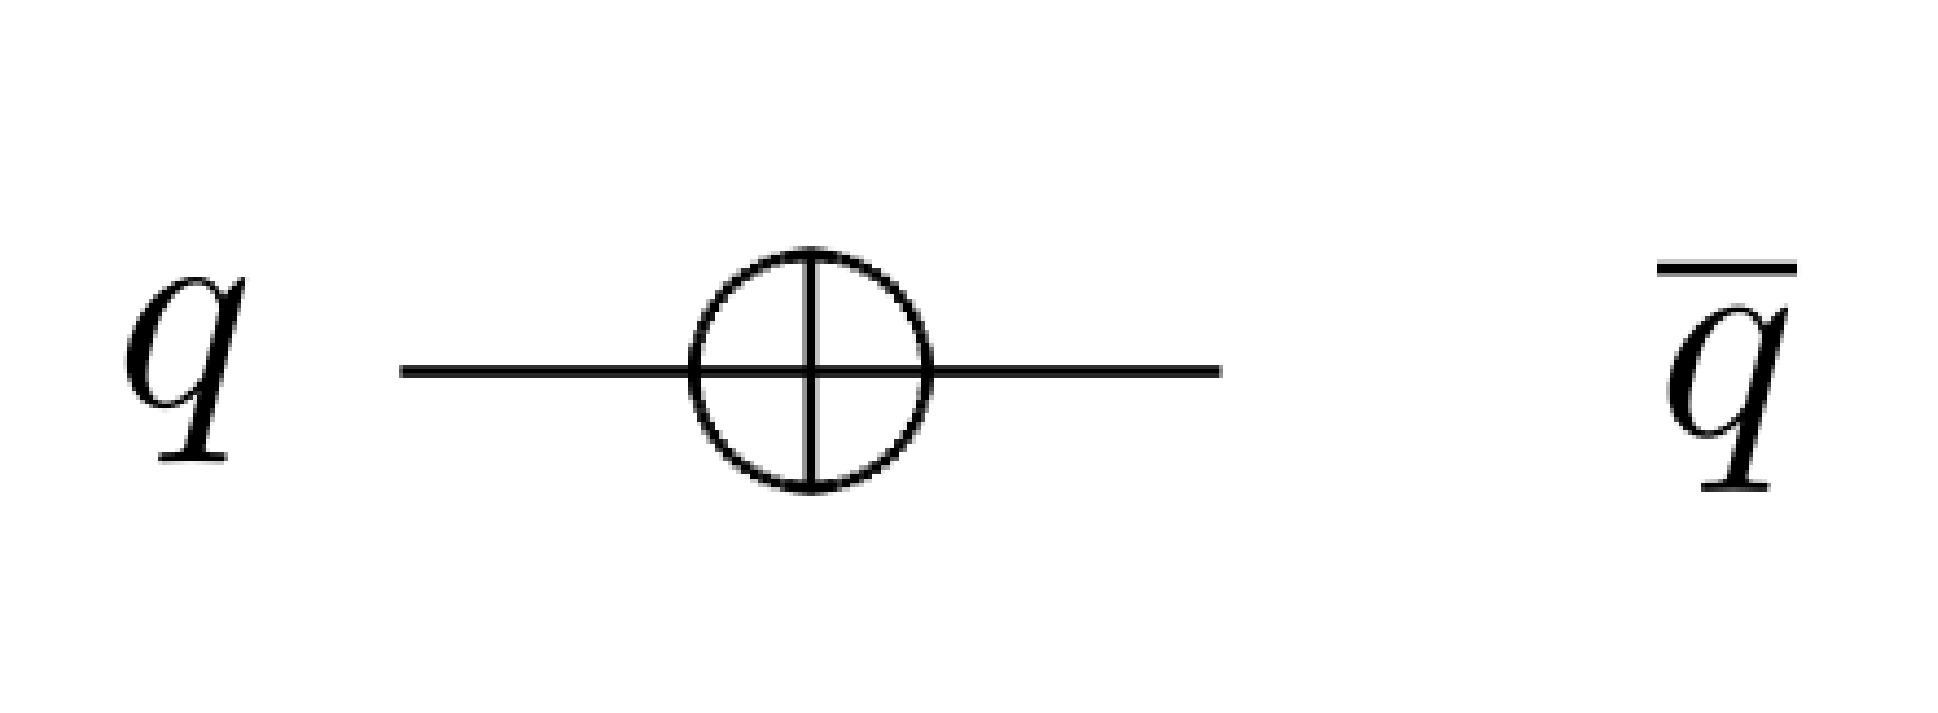
\includegraphics[width=7cm]{img/notgate.pdf}
\caption{NOT gate}
\label{not_gate}
\end{figure}
\subsection{CNOT gate}
A CNOT gate is a quantum gate that consists of one control bit and one target bit.
An example of a CNOT gate is shown in
Figure~\ref{cnot_gate}.
\begin{figure}[tbp]
\centering
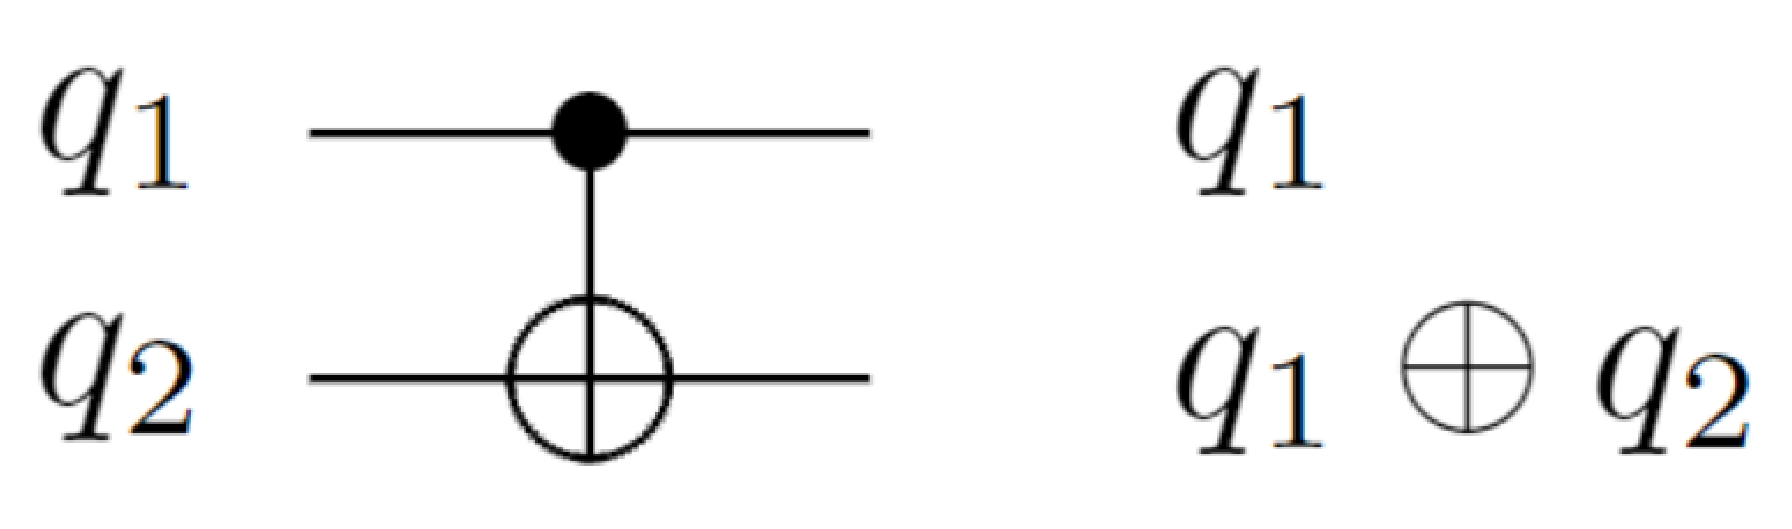
\includegraphics[width=8cm]{img/cnotgate.pdf}
\caption{CNOT gate}
\label{cnot_gate}
\end{figure}
The black circle in Figure~\ref{cnot_gate} is called the control bit,
and $\oplus$ is called the target bit.
The CNOT gate leaves the target bit unchanged when the control bit is 0, and inverts the target bit when the control bit is 1.
Since the value of the control bit never changes,
the value of the quantum bit $q_{1}$ does not change even after passing through the CNOT gate.
\subsection{T gate}
\bout{The $T$ gate is a one-qubit quantum gate that changes the phase of the quantum state by $\frac{\pi}{4}$ when the value of the qubit it acts on is 1.
\bout{The inverse transformation of the $T$ gate is called the $T^{\dag}$ gate. }
\bout{The $T^{\dag}$ gate is the inverse transformation of the $T$ gate, so when the value of the quantum bit to be acted upon is 1,
it changes the phase of the quantum state by $-\frac{\pi}{4}$. }
Examples of the $T$ gate and the $T^{\dag}$ gate are shown in Figure \ref{T_T_dag}.
\begin{figure}[tbp]
\centering
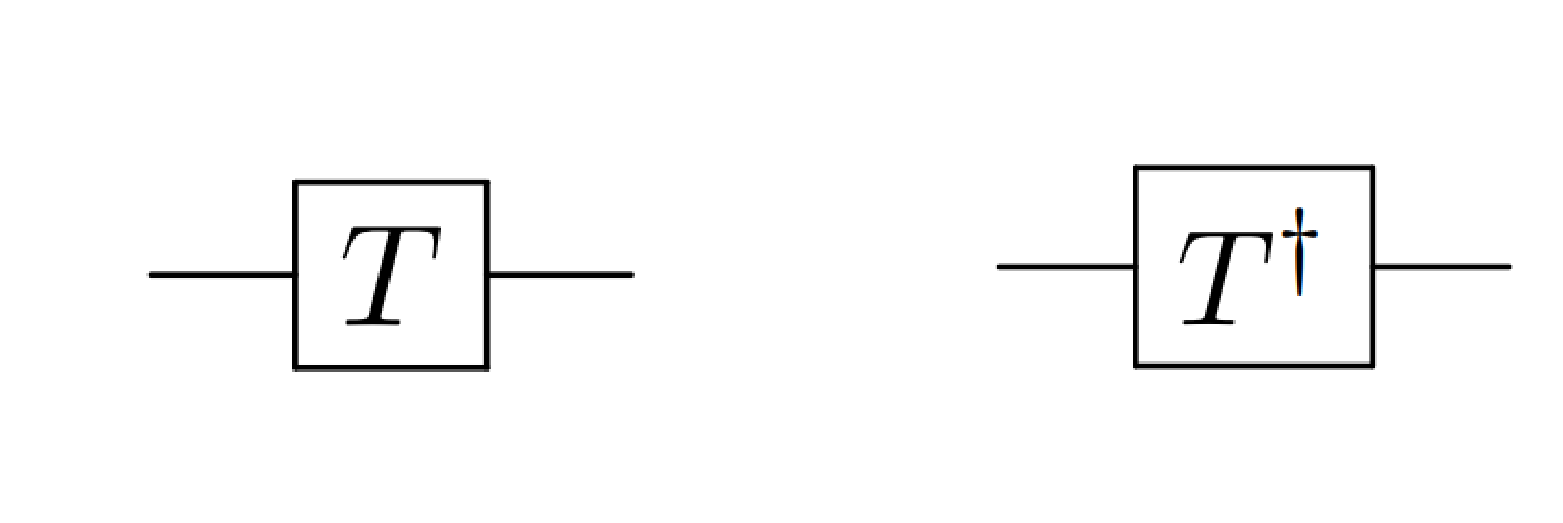
\includegraphics[width=7cm]{img/T_T_dag.pdf}
\caption{$T$ gate, $T^{\dag}$ gate}
\label{T_T_dag}
\end{figure}
\par
The operation time of the $T$ gate and the $T^{\dagger}$ gate is very long compared to other quantum gates in the Clifford+T gate group\cite{fowler2009high}.
Therefore, the number of stages of $T$ gates and $T^{\dag}$ gates that cannot be executed simultaneously in a quantum circuit is called the T-depth\cite{amy2013meet},
and reducing the value of T-depth is considered to be a challenge in quantum circuit design.
In this paper, we only consider the T-depth, so $T$ gates and $T^{\dag}$ gates are collectively called $T$ gates.
\subsection{Toffoli gate}
The Toffoli gate is a three-qubit quantum gate.
The Toffoli gate consists of two control bits and one target bit.
The Toffoli gate inverts the value of the target bit when the values of all control bits are 1.
To realize the operation of the Toffoli gate, it is necessary to decompose it into a group of Clifford+T gates.
Figure~\ref{toffoli} shows the Toffoli gate and an example of its decomposition\cite{amy2013meet}.
\par
In the decomposition example in Figure~\ref{toffoli}, three levels of $T$ gates that cannot be executed simultaneously appear.

For this reason, the T-depth of the Toffoli gate in Figure~\ref{toffoli} is 3.

\begin{figure}[tbp]

\centering

\includegraphics[width=11cm]{img/toffoli.pdf}

\caption{Toffoli gate and decomposition example into Clifford+T\cite{amy2013meet}}

\label{toffoli}

\end{figure}

\subsection{Multiple Controlled Toffoli (MCT) gate}

A generalized Toffoli gate is called the Multiple Controlled Toffoli (MCT) gate\cite{barenco1995elementary}.

The MCT gate consists of multiple control bits and one target bit.

The MCT gate inverts the value of the target bit when the values of all control bits are 1.
\par
MCT gates, like Toffoli gates, need to be decomposed into a group of Clifford+T gates.

To decompose an MCT gate with three or more control bits,
it is necessary to use bits called auxiliary bits that temporarily store values.

The auxiliary bits used here need to restore their values.

\gout{MCT gates are once decomposed into}
gates that can be decomposed into Clifford+T without auxiliary bits,
such as Toffoli gates. }
Then, the decomposed gates are decomposed into a group of Clifford+T gates.

\par
Figure~\ref{barenco} shows an example of decomposing an MCT gate with four control bits into a Toffoli gate.

\begin{figure}[tbp]
\centering
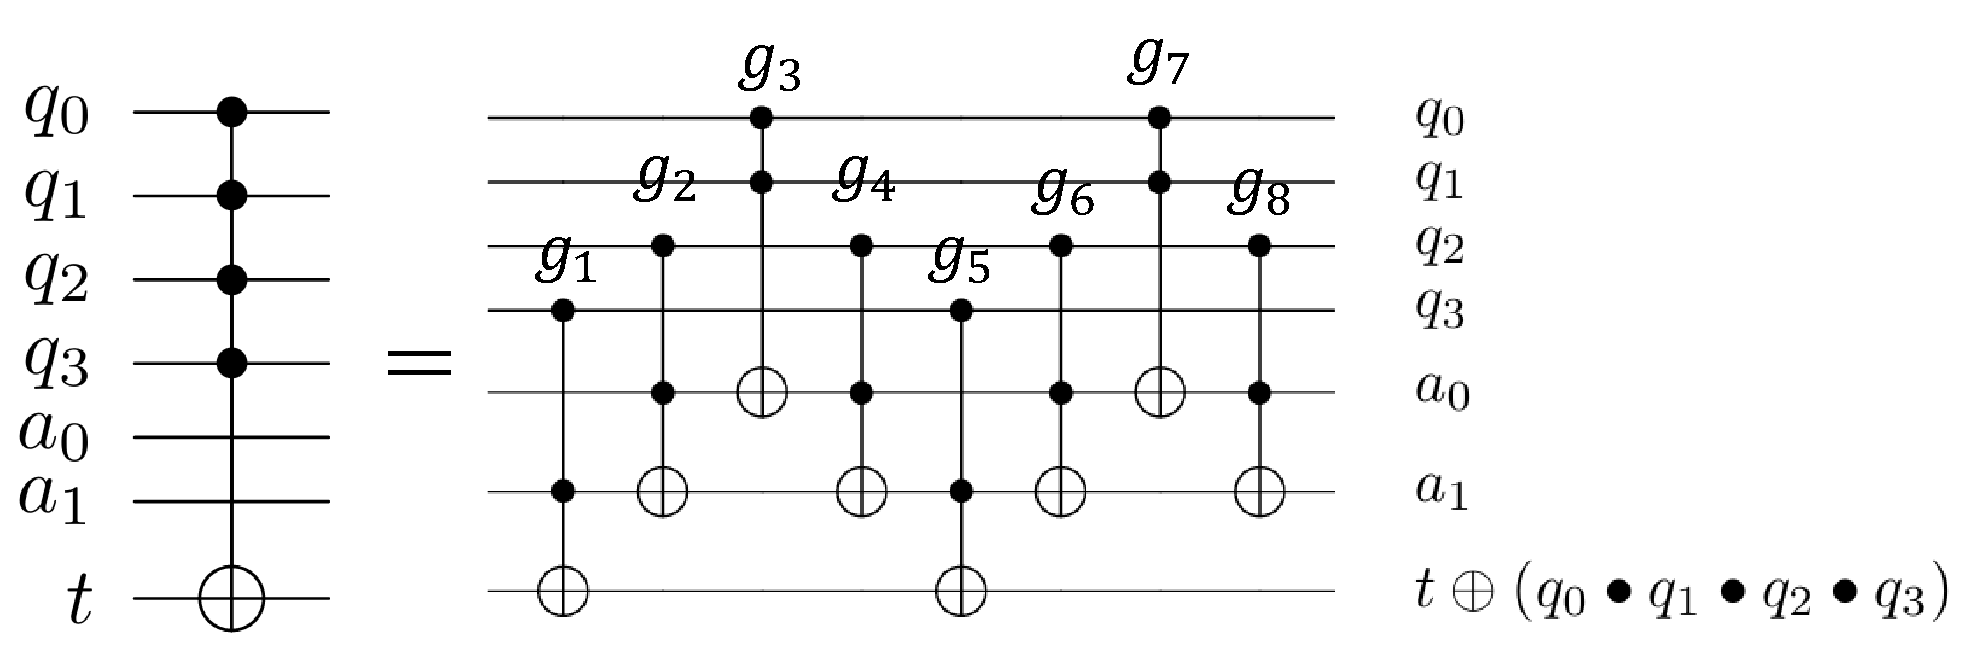
\includegraphics[width=13cm]{img/barenco.pdf}
\caption{Example of decomposition of MCT gate into Toffoli gates}
\label{barenco}
\end{figure}
In Figure~\ref{barenco}, the MCT gate is decomposed into Toffoli gates using auxiliary bits $a_{0} and a_{1}$ with undefined values.
If the number of control bits of the MCT gate is $c$, the MCT gate can be decomposed into $4(c-2)$ Toffoli gates using $c-2$ auxiliary bits with undefined values\cite{barenco1995elementary}.
In the example in Figure~\ref{barenco}, the MCT gate with 4 control bits is decomposed into 8 Toffoli gates using 2 auxiliary bits with undefined values.
\subsection{Beam Search}
Beam search\cite{bisiani1992beam} is a heuristic method for searching a tree structure while pruning.
If the tree depth is $M$ and the number of transitions from a node is $N$,
it is necessary to simulate $N^M$ possible states to examine all states.
If the values of $N$ and $M$ are large,
it is not realistic to simulate all states.
Beam search is a search algorithm that limits the search range to a predetermined number of candidates,
keeping the amount of calculations to a realistic level.
\par
In beam search,
the graph is searched by specifying the depth and width of the search in advance.
Depth means the vertical size of the tree to be searched.
Width means the horizontal size of the tree to be searched.
In beam search, the specified depth and width are searched and the best candidate is selected.
Algorithm~\ref{alg:beam_search} shows the pseudocode for beam search\bout{. }
\begin{algorithm}[tbp]
\caption{Beam search pseudocode}
\label{alg:beam_search}
\begin{algorithmic}[1]
\Require $state \Leftarrow$ Current state
\Require $legal\_actions$ Function to enumerate next transitions from state
\Require $depth \Leftarrow$ Depth to search
\Require $width \Leftarrow$ Width to search
\State $best\_state$ Best candidate
\State $candidate\_list$ List of search candidates, prioritized queue
\State $candidate\_list.push(state)$
\For{$1,,depth$}
\State $next\_candidate\_list$ List of next candidate candidates, prioritized queue
\For{$1,..,width$}
\If{If $candidate\_list$ is empty}
\State break
\EndIf
\State $now\_state \Leftarrow candidate\_list.pop()$ Extract the best value of the candidate and pop it
\State $next\_candidate\_list.push(legal\_actions(now\_state))$ Add the transition from the current state to the list of next candidate candidates
\EndFor
\State $candidate\_list \Leftarrow next\_candidate\_list$ Update the list of candidates
\State $best\_state \Leftarrow candidate\_list.top()$ Update the best candidate
\If{If $best\_state$ is the end state}
\State break
\EndIf
\EndFor
\State \Return Return the first transition of $best\_state$
\end{algorithmic}
\end{algorithm}

\begin{figure}[tbp]
\centering
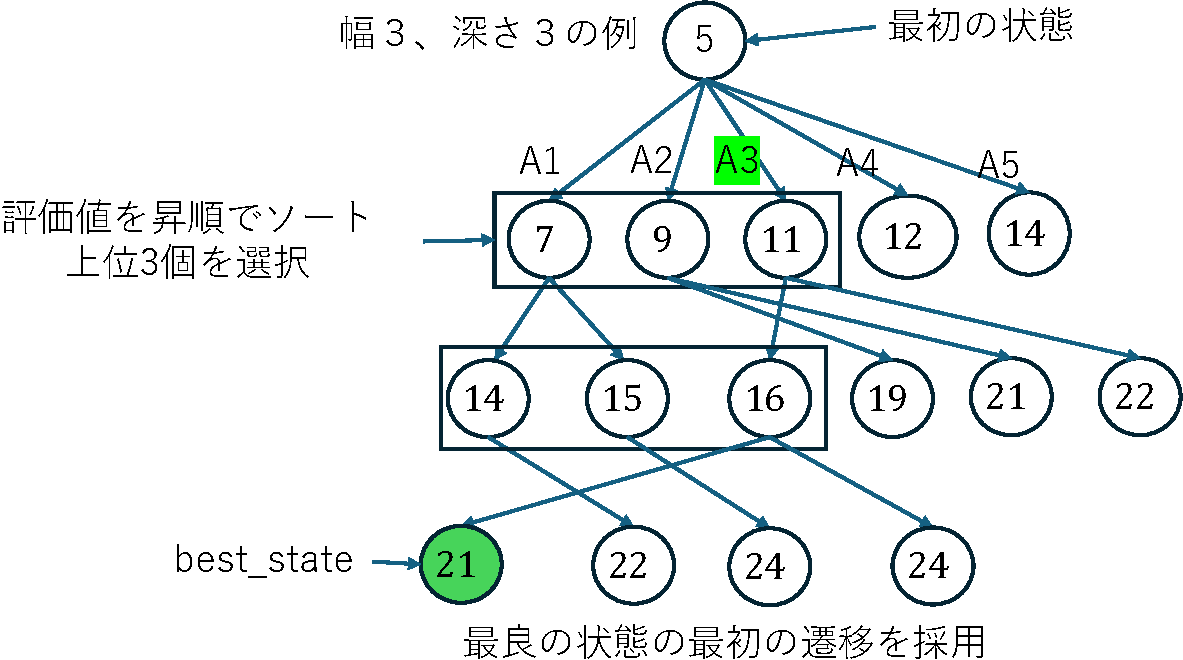
\includegraphics[width=11cm]{img/beam_search.pdf}
\caption{Example of operation of \gout{beam search} with depth 3 and width 3}
\label{beam_search}
\end{figure}
Figure~\ref{beam_search} shows an example of operation of \gout{beam search} with depth 3 and width 3.
In Figure~\ref{beam_search}, each node represents a state.
The number written on the node represents the evaluation value of that state.
In the example of \gout{Figure~\ref{beam_search}}, the solution with the smallest evaluation value is considered to be the better solution.
The state transitions from the initial state are A1, A2, \dots, and A5.
In Figure~\ref{beam_search}, the transitions from the initial state to five states are listed.
Since the search width is 3, the top 3 states are searched.

From the top 3 states, \gout{list the states that transition to} and then search the top 3 states again.

This process is repeated, and when a depth of 3 is reached, the first transition A3 that is the best candidate at that time is adopted.

\section{Decomposition method of MCT gates}
In this chapter, we explain the existing \bout{decomposition method\cite{abdessaied2016technology,baker2019decomposing,niemann2019t}} of MCT gates.

Hereafter, the number of control bits of MCT gates is $c$.

\subsection{Method~1}
In this section, we explain the decomposition method \cite{abdessaied2016technology} of MCT gates that uses $c-2$ auxiliary bits with indefinite values.

Hereafter, this method will be called Method~1.

\bout{Method~1}
is a method to reduce the T-depth of the method \cite{barenco1995elementary} that decomposes MCT gates into Toffoli gates.

In Method~1, the T-depth is reduced by replacing Toffoli gates with out-of-phase $CCiZ, CCi\omega Z$ gates.
\par
After decomposing MCT gates into Toffoli gates,
we explain how to replace these Toffoli gates with $CCiZ$ gates and $CCi\omega Z$ gates.
In method 1, we first replace Toffolli gates with $CCZ$ gates and H gates.
As shown in Figure~\ref{toffoli_transform}, Toffoli gates can be replaced with H gates and $CCZ$ gates.
For this reason, the Toffoli gates in Figure barenco can be replaced with $CCZ$ gates and H gates as shown in Figure~\cite{toffoli_to_ccz} \begin{figure}[tbp] \centering \begin{minipage}[b]{0.8\columnwidth} \centering 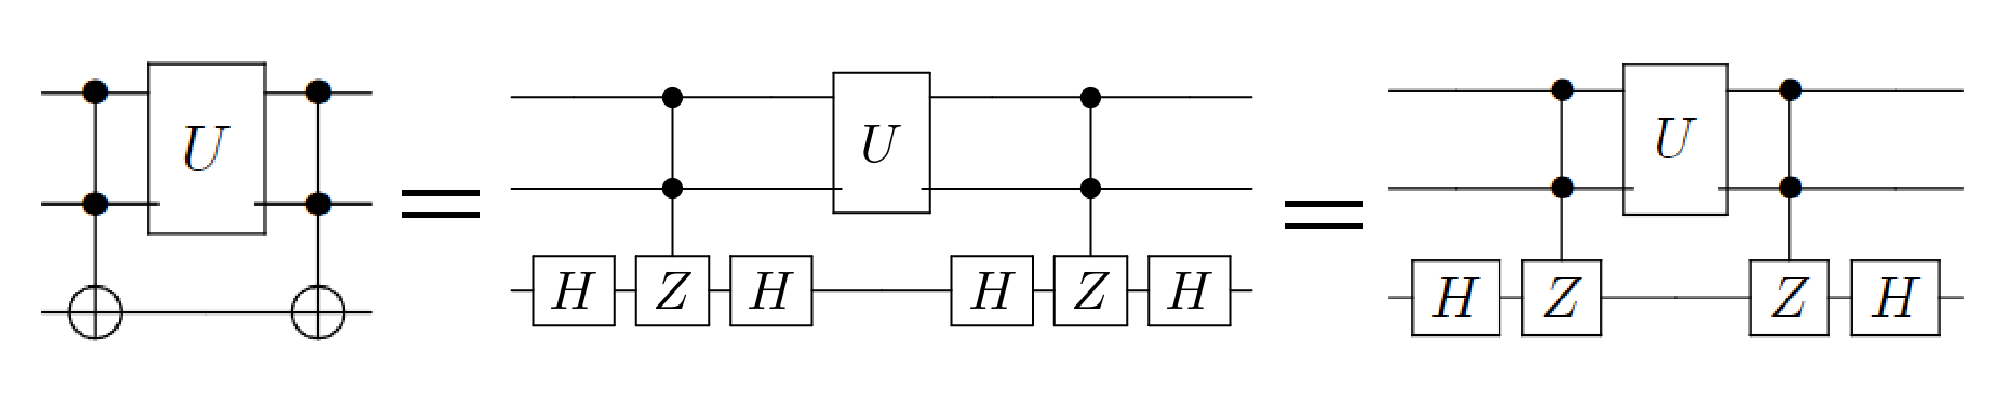
\includegraphics[width=0.9\columnwidth]{img/toffoli_transform.pdf} \caption{Replacement of Toffoli gate with $CCZ$ gate} \label{toffoli_transform} \end{minipage} \begin{minipage}[b]{0.4\columnwidth} \centering 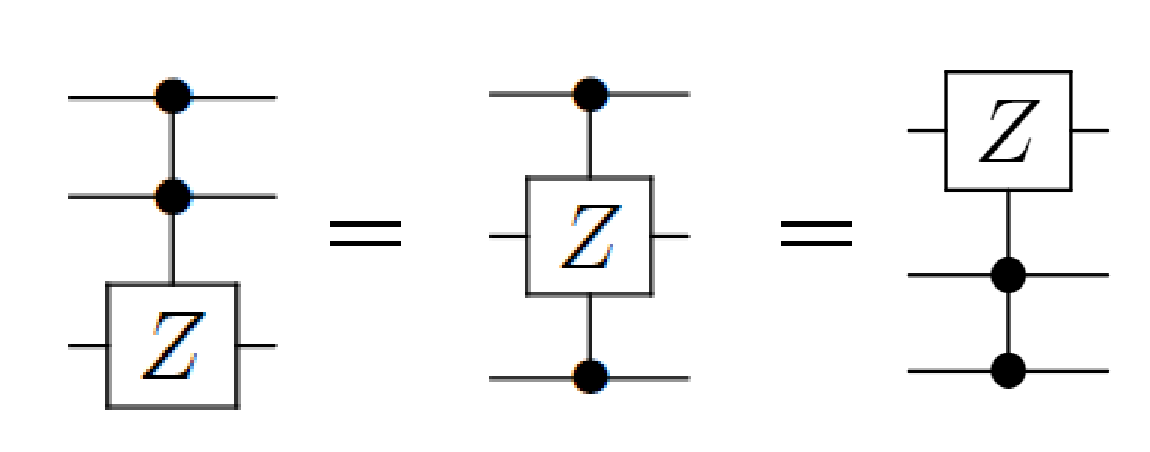
\includegraphics[width=0.9\columnwidth]{img/zgate_transform.pdf} \caption{$CCZ$gate transformation} \label{zgate_transform} \end{minipage} \end{figure} \begin{figure}[tbp] \centering 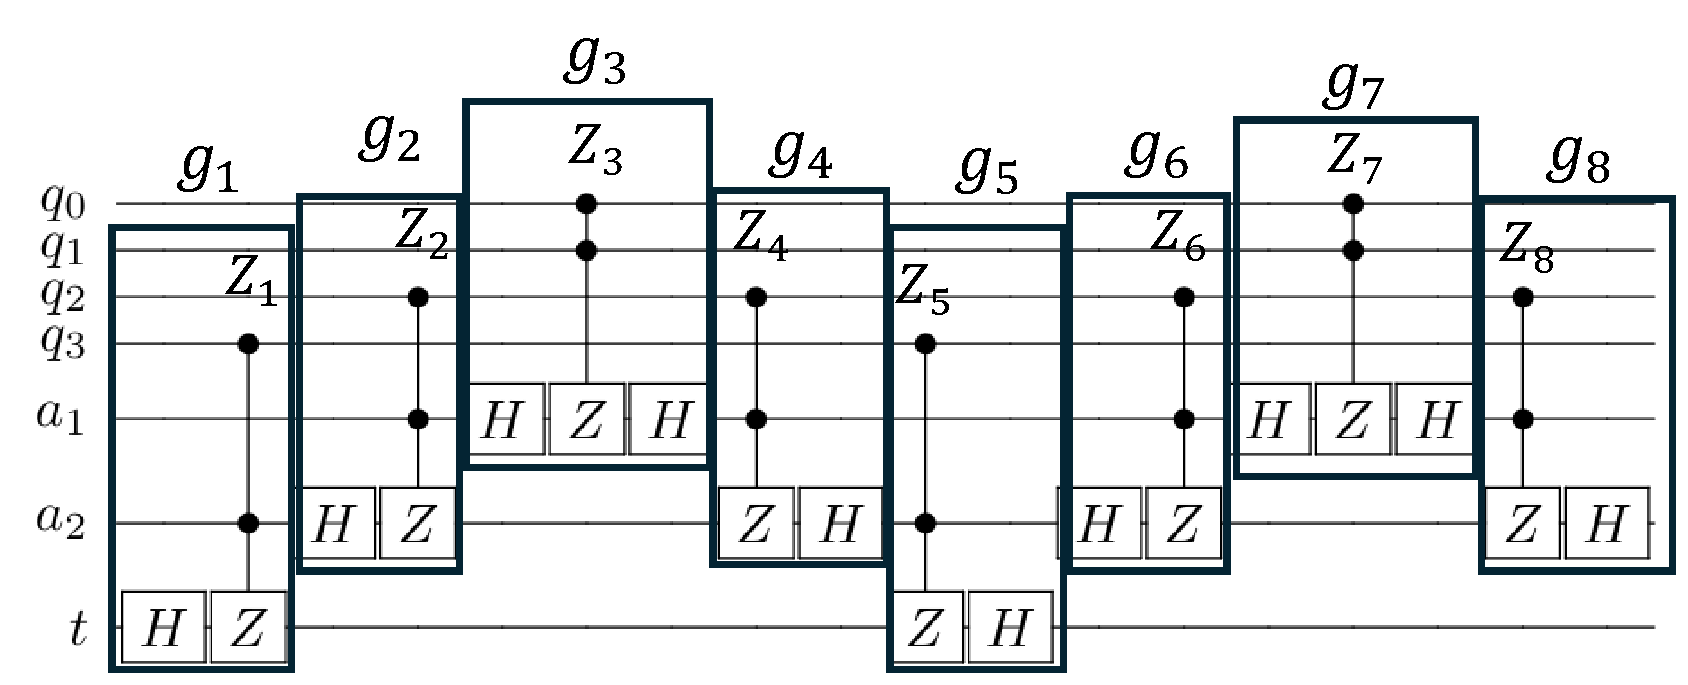
\includegraphics[width=13cm]{img/toffoli_to_ccz.pdf} \caption{An example of replacing the Toffoli gate in Figure~\ref{barenco} with a $CCZ$ gate and an H gate}
\label{toffoli_to_ccz}
\end{figure}
\par
\mout{Next, we explain how to replace the replaced $CCZ$ gate with a $CCiZ$ gate.
As shown in Figure~\ref{zgate_transform}, the $CCZ$ gate can be considered to have the same control bit and target bit.
Also, as shown in Figure~\ref{zgate_to_iz}, the $CCZ$ gate can be replaced with
$CCiZ, CS$ gates or $CCiZ^{\dag}, CS^{\dag}$ gates.
For this reason, as shown in Figure~\ref{ccz_to_iz_cs}, the $CCZ$ gate in Figure~\ref{toffoli_to_ccz} can be replaced with $CCiZ, CS$ gates and $CCiZ^{\dag}, CS^{\dag}$ gates.

In Figure~\ref{ccz_to_iz_cs}, the pairs of
opposing gates $\{Z_{1}. Z_{5}\}, \{Z_{2}, Z_{4}\}, \{Z_{3}, Z_{7}\},\{Z_{6}, Z_{8}\}$
in Figure~\ref{toffoli_to_ccz} are replaced with pairs of $CCiZ, CS$ gates and $CCiZ^{\dag}, CS^{\dag}$ gates, respectively.

When replacing these opposing $CCZ$ gates,
they are replaced so that no operations occur between the $CS and CS^{\dag}$ gates after replacement.
For example, for the pair $Z_{3} and Z_{7}$,
the replacement is performed so that the control bit of the $CS and CS^{\dag}$ gates becomes $q_{0}$ and the target bit becomes $q_{1}$ so that no operations occur between the $CS and CS^{\dag}$ gates after replacement.
The $CS and CS^{\dag}$ gates arranged as in Figure~\ref{izgate_transform} can be deleted because their operations cancel each other out.
For this reason, the opposing $CS and CS^{\dag}$ gates, $S_{1}, \dots, and S_{8}$ in Figure~\ref{ccz_to_iz_cs}, which have no operations between them, can be deleted.
In this way, the $CCZ$ gates can be replaced with $CCiZ$ gates. }
\begin{figure}[tbp]
\centering
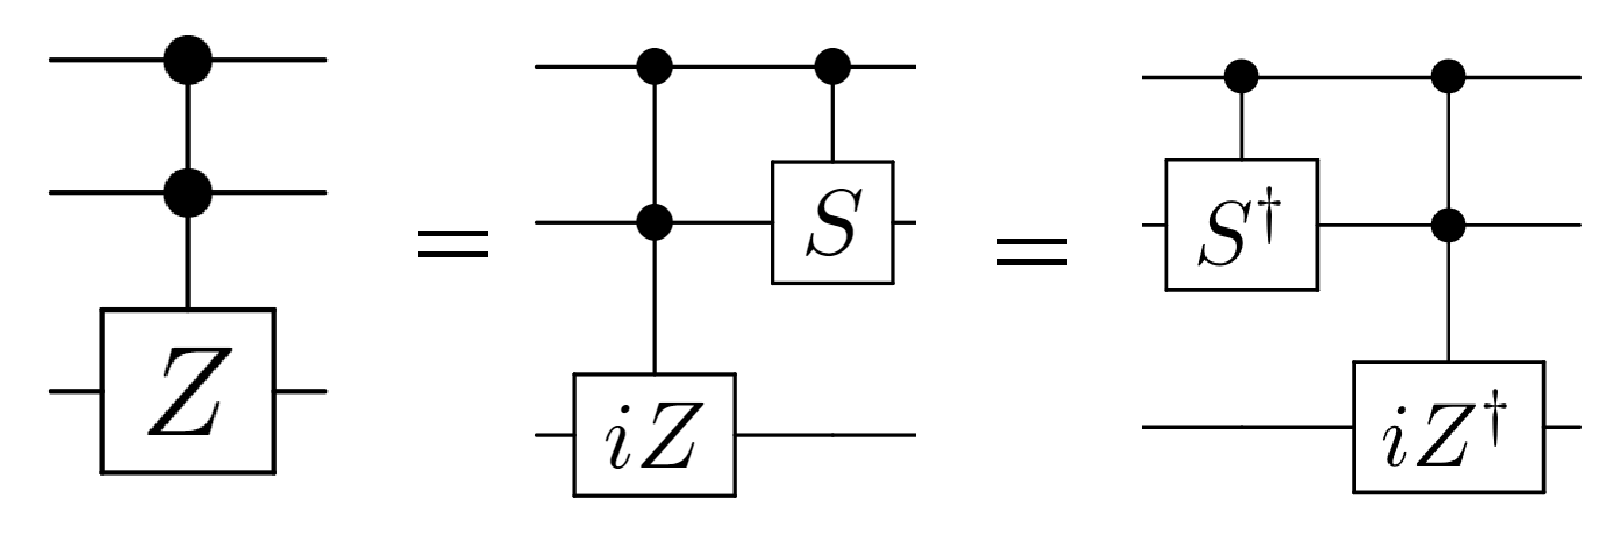
\includegraphics[width=0.5\columnwidth]{img/zgate_to_izgate.pdf}
\caption{Replacement of $CCZ$ gates to $CCiZ, CS$ gates, $CCiZ^{\dag}, CS^{\dag}$ gates}
\label{zgate_to_iz}
\end{figure}
\begin{figure}[tbp]
\centering
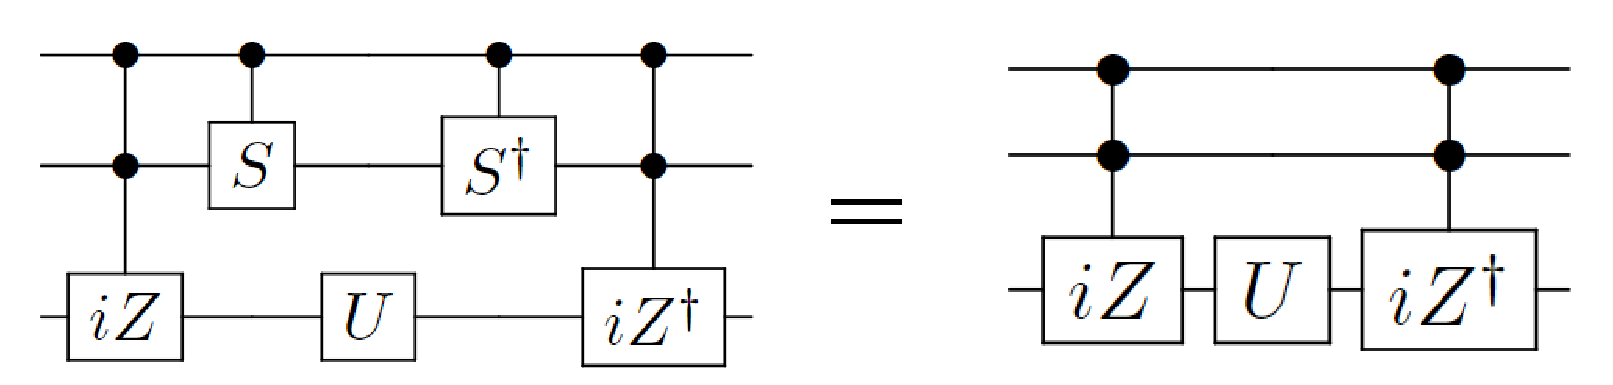
\includegraphics[width=0.5\columnwidth]{img/izgate_transformation.pdf}
\caption{Cancellation of $CS, CS^{\dag}$ gates}
\label{izgate_transform}
\end{figure}
\begin{figure}[tbp]
\centering
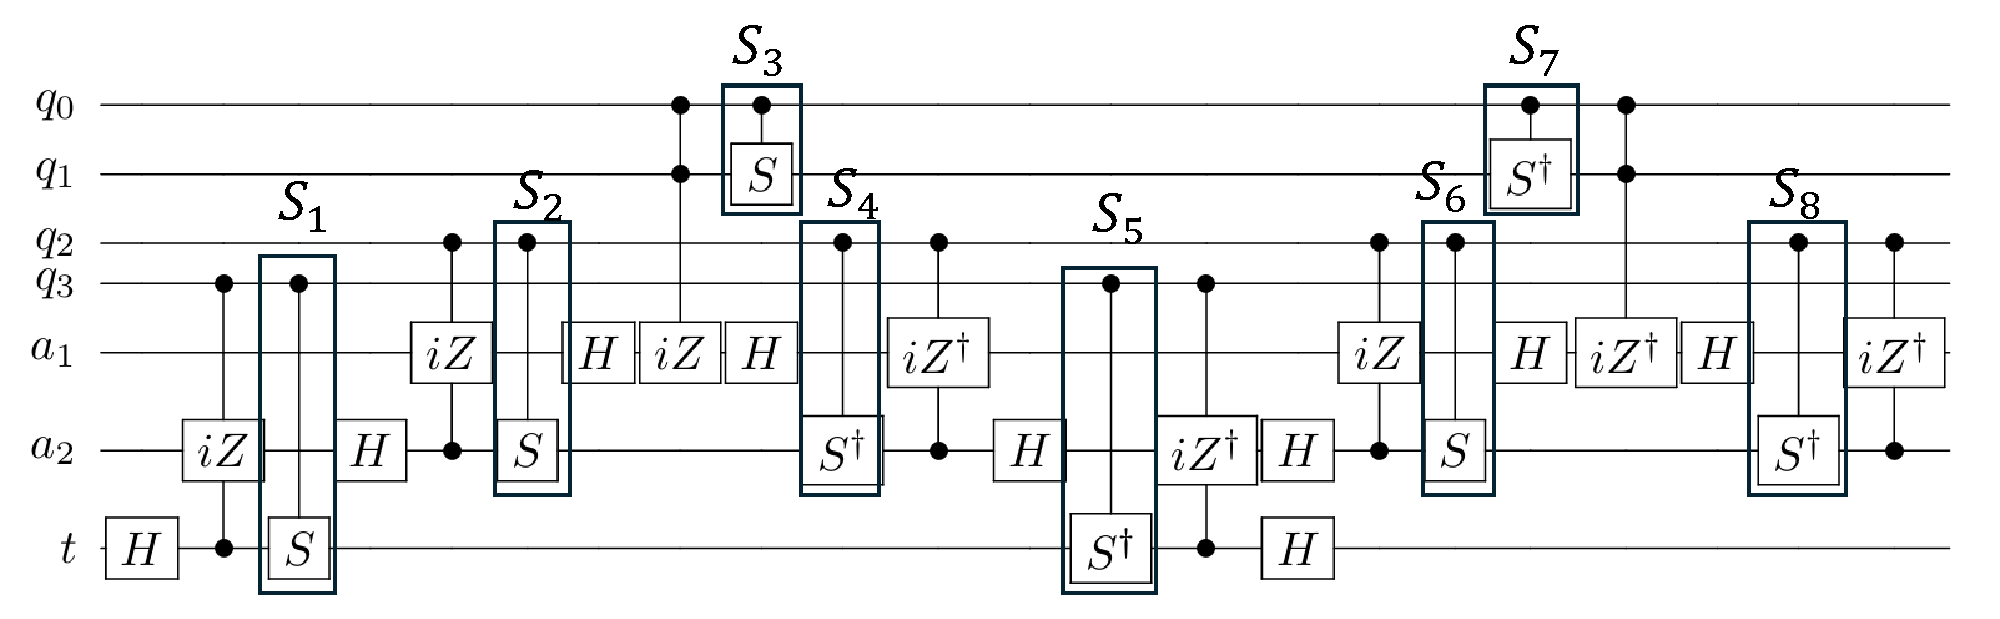
\includegraphics[width=14cm]{img/ccz_to_iz_cs.pdf}
\caption{An example of replacing the $CCZ$ gate in Figure~\ref{toffoli_to_ccz} with $CCiZ, CS$ gates and $CCiZ^{\dag}, CS^{\dag}$ gates}

\label{ccz_to_iz_cs}
\end{figure}
\par
\mout{Finally, we explain how to replace the $CCiZ$ gate with a $CCi\omega Z$ gate.
As shown in Figure~\ref{iz_to_iomegaz}, the $CCiZ$ gate can be replaced with a $CCi\omega Z$ gate and a $T^{\dag}$ gate,
and the $CCiZ^{\dag}$ gate can be replaced with a $CCi\omega Z^{\dag}$ gate and a $T$ gate.
Figure~\ref{barenco_iz_to_iomegaz} shows an example in which the $CCiZ, CCiZ^{\dag}$ gates in Figure~\ref{ccz_to_iz_cs} are replaced with $CCi\omega Z, T^{\dag}$ gates and $CCi\omega Z^{\dag}, T$ gates, respectively.

The $T_{2}$ and $T_{3}$ gates in Figure~\ref{barenco_iz_to_iomegaz} cancel each other out,
so these $T, T^{\dag}$ gates can be deleted.

The $T_{4}$ in Figure~\ref{barenco_iz_to_iomegaz} restores the operation of $T_{1}$.

These gates can be deleted because their absence does not affect the results of the calculation.
In this way, we delete the $T and T^{\dag}$ gates, which have no effect on the calculation, and replace the $CCiZ$ gate with a $CCi\omega Z$ gate.

As a result,
as shown in Figure~\ref{techmap},
the gates $g_{1} and g_{5}$ located at the bottom and the gates $g_{3} and g_{7}$ located at the top in Figure~\ref{barenco} can be replaced with $CCiZ and CCiZ^{\dag}$ gates.

Furthermore, the gates $g_{2} and g_{4}$ and $g_{6} and g_{8}$ in Figure~\ref{barenco} can be replaced with $CCi\omega Z and CCi\omega Z^{\dag}$ gates, respectively. }
\begin{figure}[tbp]
\centering
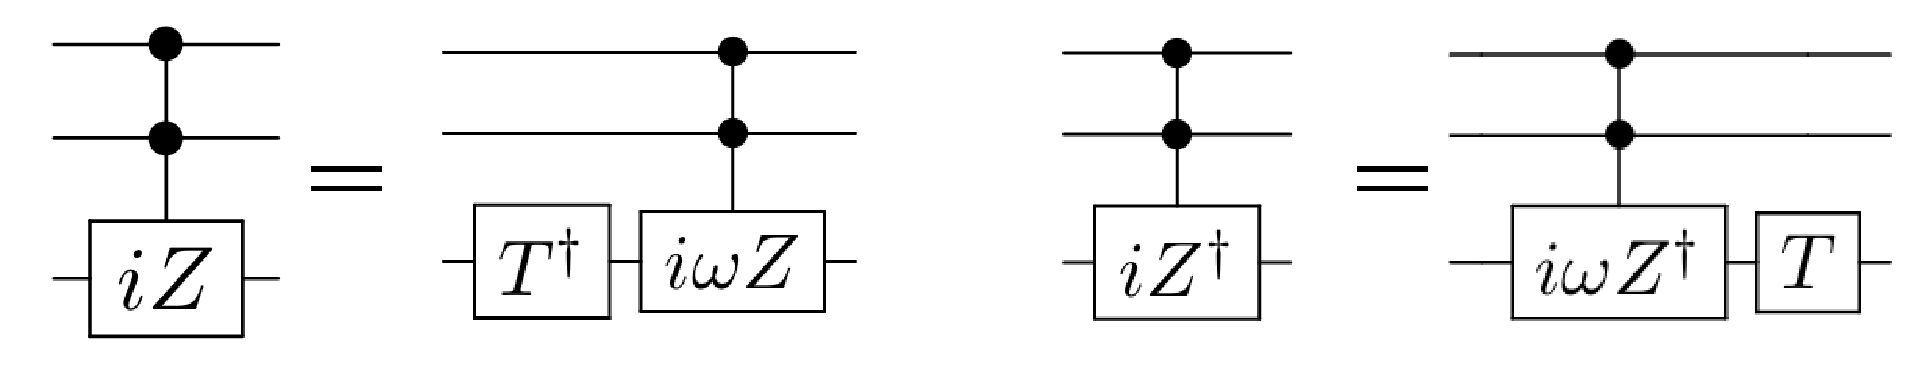
\includegraphics[width=11cm]{img/iz_to_iomegaz.pdf}
\caption{\bout{Replacement of $CCiZ$ gate with $CCi\omega Z, T^{\dag}$ gate, and replacement of $CCiZ^{\dag}$ gate with $CCi\omega Z^{\dag}, T$ gate}}
\label{iz_to_iomegaz}
\end{figure}
\begin{figure}[tbp]
\centering
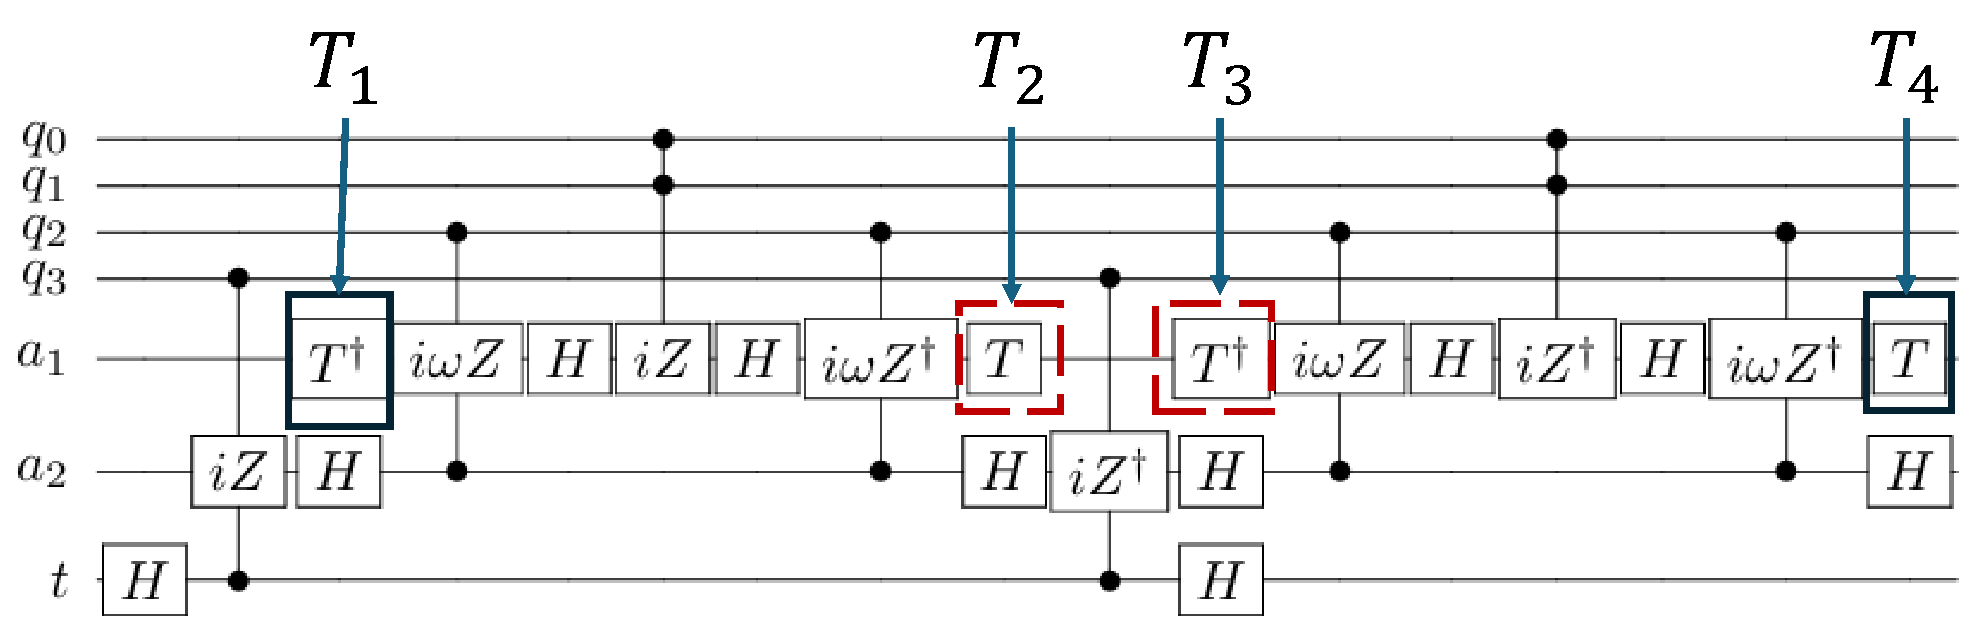
\includegraphics[width=14cm]{img/barenco_iz_to_iomegaz.pdf}
\caption{Replacement of $CCiZ$ and $CCiZ^{\dag}$ gates in Figure~\ref{ccz_to_iz_cs} with $CCi\omega Z, T^{\dag}$ gates, respectively.}

\label{barenco_iz_to_iomegaz}

\end{figure}

\begin{figure}[tbp]

\centering

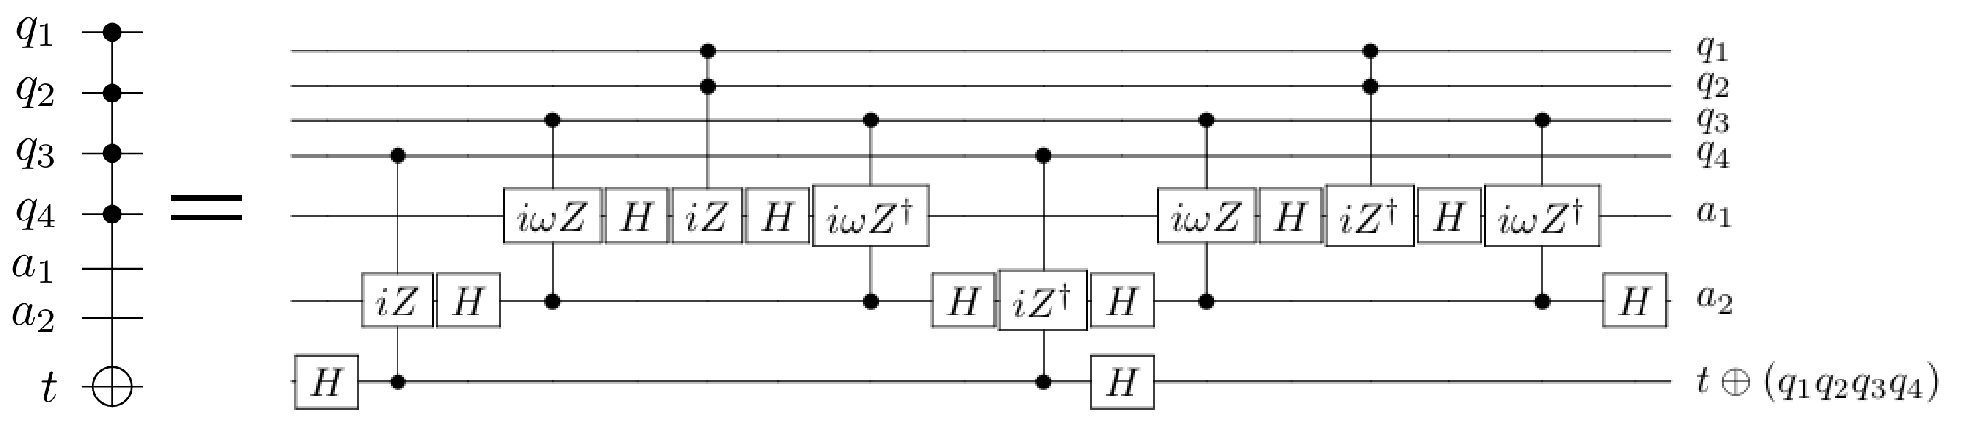
\includegraphics[width=0.9\columnwidth]{img/techmap.pdf}

\caption{Application of method 1 to MCT gates with $c=4$}

\label{techmap}

\end{figure}

\par
Method 1 uses $c-2$ auxiliary bits to decompose the MCT gate into 4 $CCiZ$ gates and $4(c-3)$ $CCi\omega Z$ gates.

The decomposition of the $CCiZ$ gate and the $CCi\omega Z$ gate into Clifford+T is shown in Figure 1 and Figure 2, respectively.

The T-depth of the $CCiZ$ gate is 2, and the T-depth of the $CCi\omega Z$ gate is 1.

Therefore, the maximum T-depth of the MCT gate decomposed by method 1 is $4(c-1)$.

\begin{figure}[tbp]

\centering

\begin{minipage}[b]{0.49\columnwidth}

\centering

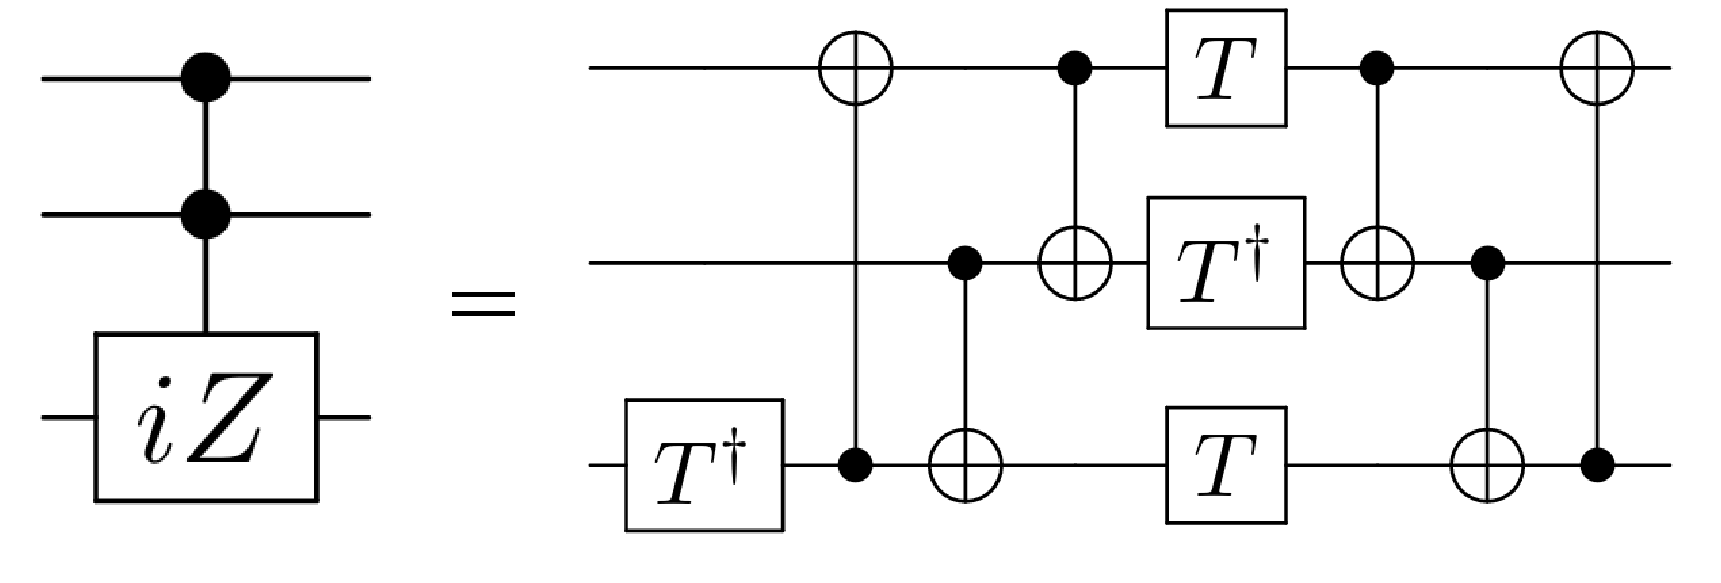
\includegraphics[width=0.9\columnwidth]{img/cciz.pdf}

\caption{Decomposition of $CCiZ$ gate into Clifford+T}

\label{cciz}

\end{minipage}

\begin{minipage}[b]{0.49\columnwidth}

\centering

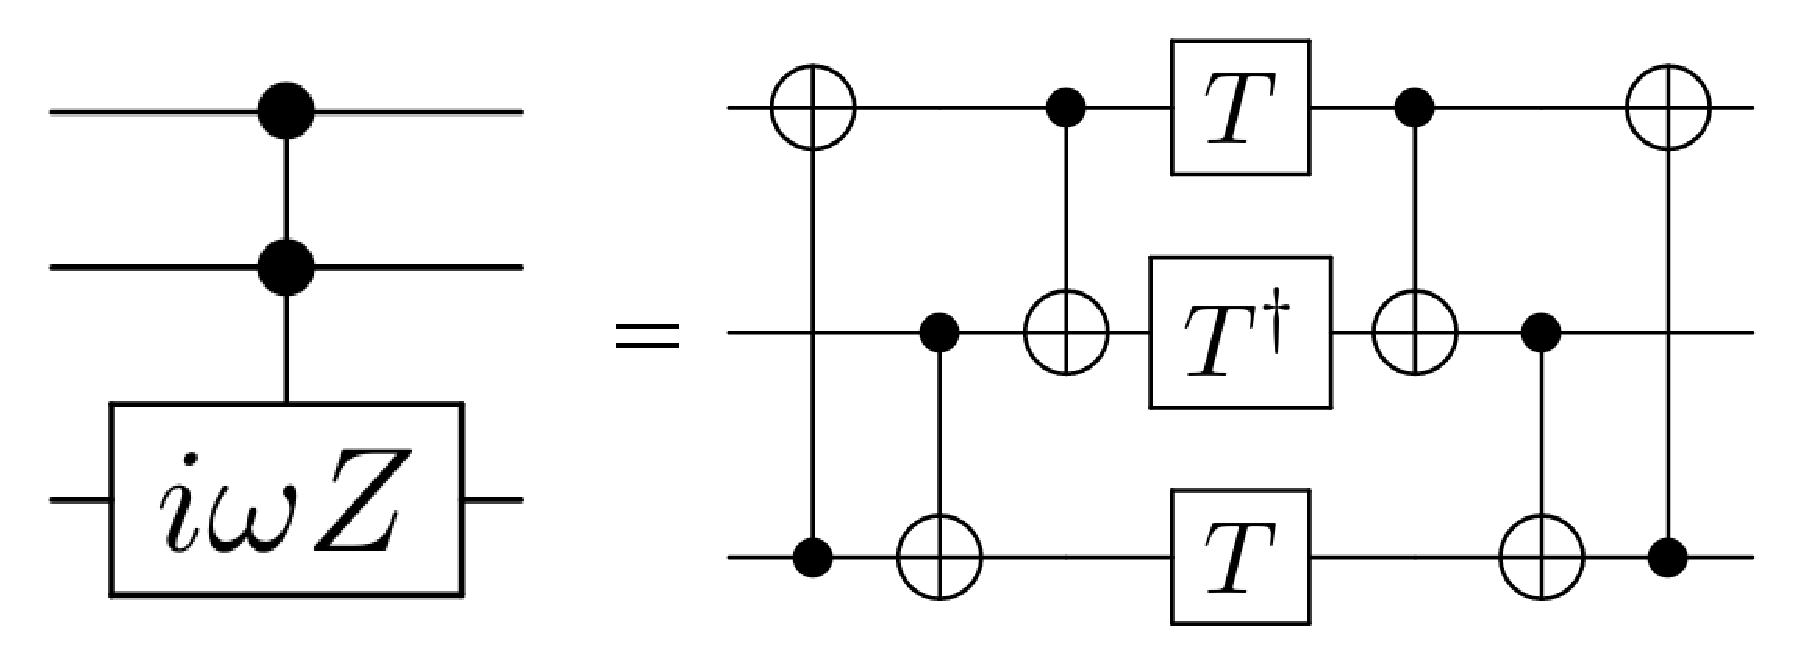
\includegraphics[width=0.9\columnwidth]{img/cciomegaz.pdf}

\caption{$Decomposition of CCi\omega Z$ gate into Clifford+T}
\label{cciomegaz}
\end{minipage}
\end{figure}
\subsection{Method~2}
In this section, we explain the decomposition method \cite{abdessaied2016technology} that uses one auxiliary bit with an undefined value.
Hereafter, we will refer to this method as Method~2.
\par
When there are fewer than $c-2$ auxiliary bits with undefined values, the MCT gate cannot be decomposed using Method~1.
%We explain how to decompose the control bits into two.
\bout{Therefore, we divide the $c$ control bits into two sets of bits.
At this time, we divide them so that the difference in the number of elements in the two sets of bits is within one. }
Then, as shown in Figure~\ref{mimap},
the MCT gate is decomposed into four MCT gates,
$g_{1}, g_{2}, g_{3}, g_{4}$, and four $C\omega S$ gates,
which have the set of split bits as their control bits.
\begin{figure}[tbp]
\centering
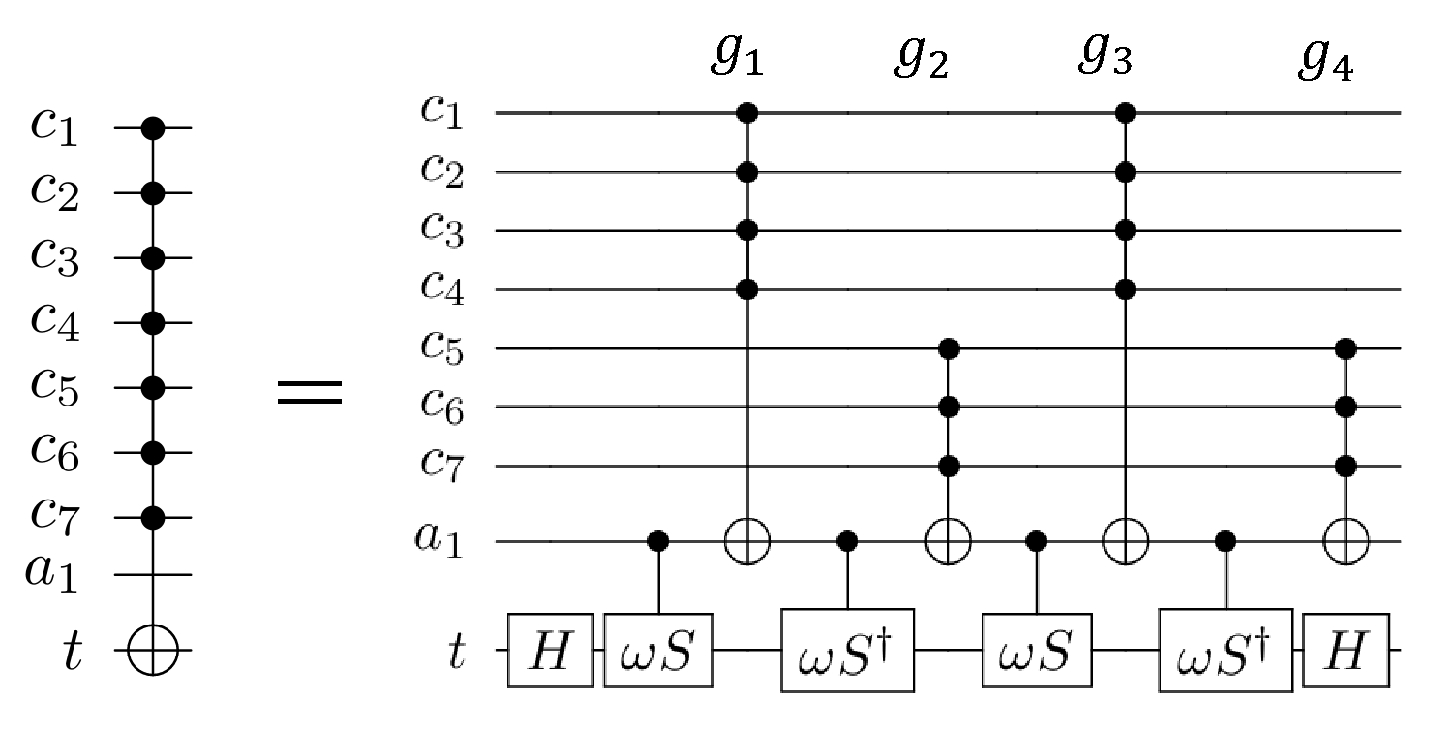
\includegraphics[width=11cm]{img/mimapping.pdf}
\caption{Application of method~2 to MCT gate with $c=7$}
\label{mimap}
\end{figure}
Here, $g_{3}$ is a copy of $g_{1}$, and $g_{4}$ is a copy of $g_{2}$.
\begin{figure}[tbp]
\centering
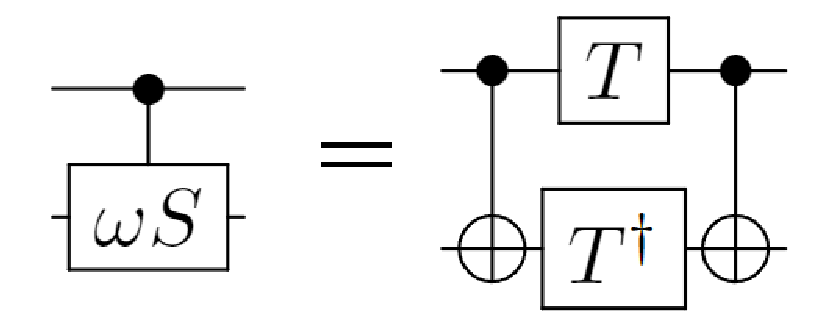
\includegraphics[width=5cm]{img/comegas.pdf}
\caption{Decomposition of $C\omega S$ gate into Clifford+T}
\label{comegas}
\end{figure}
As shown in Figure~\ref{comegas},
the $C\omega S$ gate can be decomposed directly into Clifford+T without using auxiliary bits.
In Method~2,
by applying Method~1 to the four decomposed MCT gates,
the MCT gate can be decomposed into Clifford+T.
\par
In Method~2,
the same auxiliary bits are used to replace $g_{3}$ in Figure~\ref{mimap} with the decomposition of $g_{1}$, and $g_{4}$ with the decomposition of $g_{2}$,
and the T-depth is reduced by decomposing in the reverse order.
\mout{
Figure~\ref{mimap_g2_g4}
shows an example of decomposing $g_{2}$ in Figure~\ref{mimap},
replacing $g_{4}$ with gates of the inverse transformation for the decomposition of $g_{2}$, and decomposing in the reverse order.
$G_{2} and G_{4}$ in Figure~\ref{mimap_g2_g4} represent the decomposition of $g_{2} and g_{4}$.
$G_{4}$ is the gates that make up $G_{2}$ replaced with gates of the inverse transformation, and decomposed in the reverse order. }
\begin{figure}[tbp]
\centering
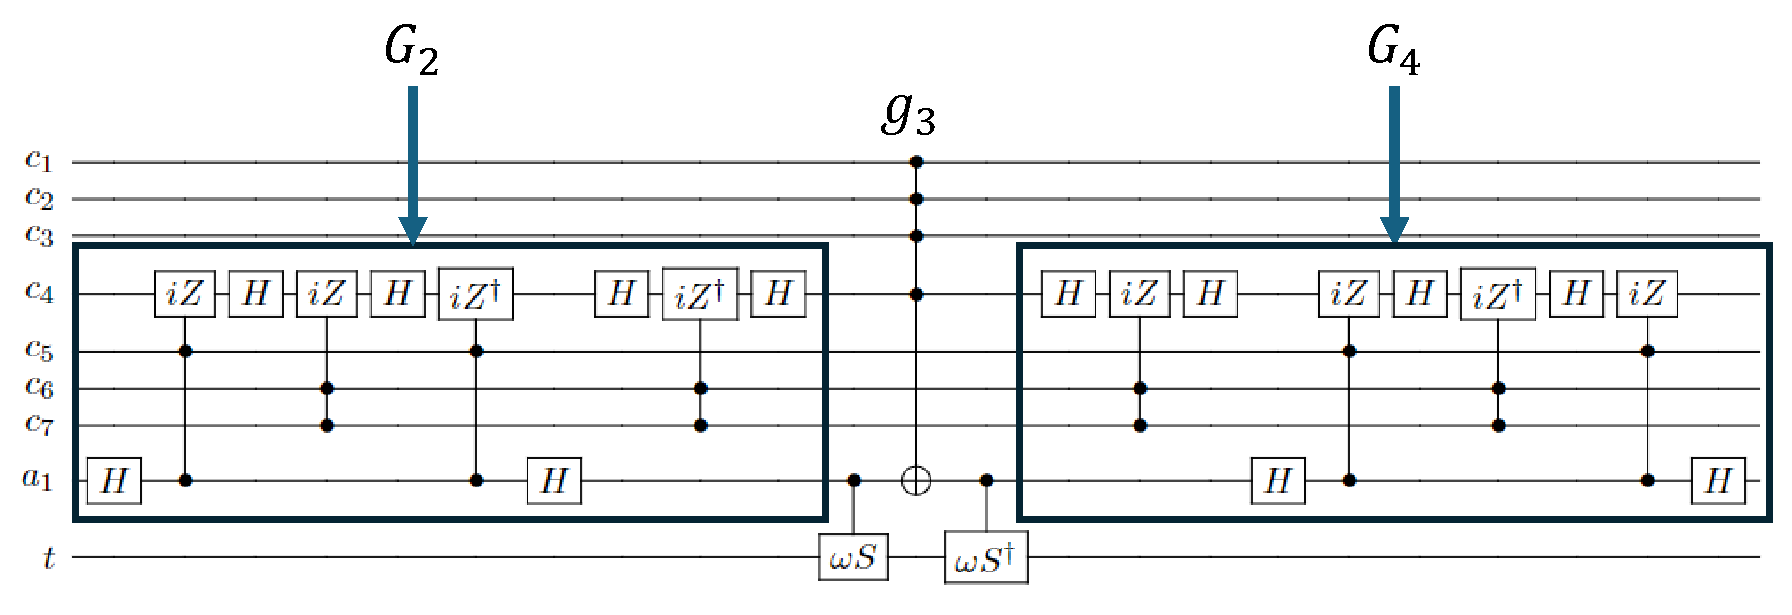
\includegraphics[width=15cm]{img/mimap_g2_g4.pdf}
\caption{\mout{An example of decomposing $g_{2}$ in Figure~\ref{mimap}, replacing $g_{4}$ with a gate that is the inverse transformation of the decomposition of $g_{2}$, and decomposing in the reverse order}}
\label{mimap_g2_g4}
\end{figure}
As shown in Figure~\ref{iz_to_iomegaz},
\bout{The $CCiZ gate$ and $CCiZ^{\dag}$ gate can be replaced by the $CCi\omega Z, T^{\dag}$ gate and the $CCi\omega Z^{\dag}, T$ gate, respectively. }
Figure~\ref{mimap_g2_g4_trans} shows an example in which the \bout{$CCiZ gate$ and $CCiZ^{\dag}$ gate in Figure~\ref{mimap_g2_g4} are replaced with the $CCi\omega Z, T^{\dag}$ and $CCi\omega Z^{\dag}, T$ gates, respectively}

.
\mout{
The $T$ gate $T_{4}$ in Figure~\ref{mimap_g2_g4_trans} restores the operation of the $T^{\dag}$ gate $T_{1}$.

These gates can be deleted because their absence does not affect the results of the calculation.

Similarly, $T_{2} and T_{3}$ in Figure~\ref{mimap_g2_g4_trans} can also be deleted.}
\par
In this way, by decomposing the pair $g_{1}, g_{3}$ and the pair $g_{2}, g_{4}$,
a total of eight $CCiZ, CCiZ^{\dag}$ gates can be replaced with $CCi\omega Z, CCi\omega Z^{\dag}$ gates, and the T-depth can be reduced by 8 from before the substitution.

To allow one difference in the control bits and divide evenly,
the total T-depth of the four MCT gates before the substitution when decomposed using method 1 is
$2 \cdot 4(\lfloor \frac{c}{2} \rfloor -1) +2\cdot 4(\lceil \frac{c}{2} \rceil -1)=8(c-1)$.

In addition, because four $C\omega S$ gates are used, the total T-depth of these gates is $4$. 
Therefore, when an MCT gate with $c$ control bits is decomposed using method 2, the maximum T-depth is $8(c-1)-8+4=8c-20$.
\begin{figure}[tbp]
\centering
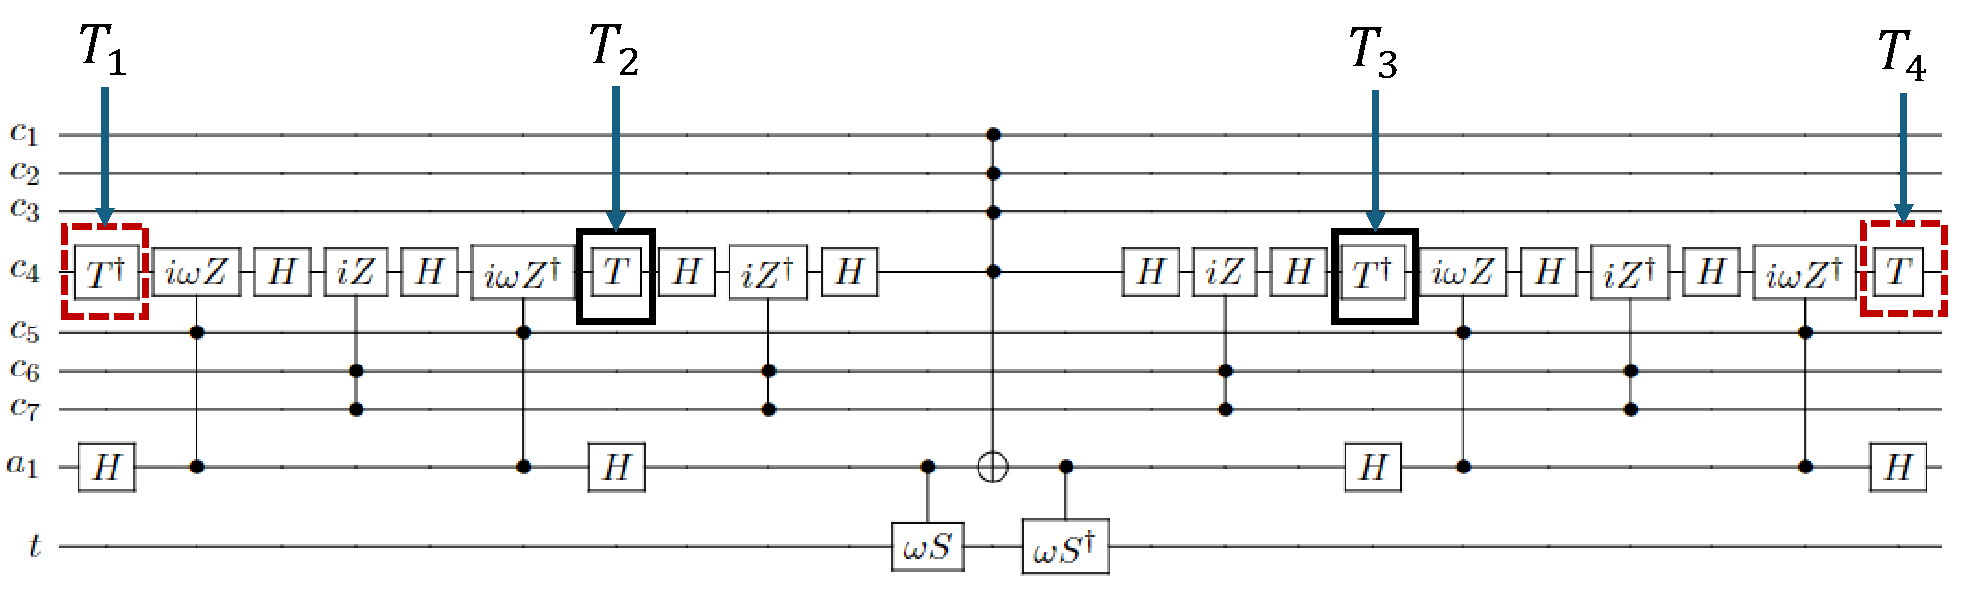
\includegraphics[width=18cm]{img/mimap_g2_g4_transform.pdf}
\caption{Figure~\ref{mimap_g2_g4}\bout{An example of replacing the $CCiZ and CCiZ^{\dag}$ gates with $CCi\omega Z, T^{\dag}$ gates and $CCi\omega Z^{\dag}, T$ gates, respectively}}
\label{mimap_g2_g4_trans}
\end{figure}
\subsection{Method~3}
In this section, we explain the method\cite{baker2019decomposing}, which uses 2 to $c-3$ auxiliary bits with indefinite values to decompose MCT gates.
Hereafter, we will refer to this method as Method~3.
As shown in Figure~\ref{baker},

Method~3 is a method to reduce T-depth by decomposing MCT gates $g_{1}$ or $g_{4}$, which require a small number of copies, using many control bits.

In Figure~\ref{baker}, $g_{1}$ has only $g_{7}$ copies,

but $g_{2}$ has $g_{6}, g_{8}, and g_{13}$ copies,

so $g_{1}$ can be said to be a gate with a small number of copies.

For $g_{4}$, the only copy is $g_{10}$.

\par
The decomposition method of Method~3 is explained below.

Let $C$ be a set of $c$ control bits of the MCT gate to be decomposed.

Let $t$ be the target bit of the MCT gate to be decomposed.
\mout{Let $a_{1}, a_{2}, \dots, a_{m}$ be the $m$ auxiliary bits with indefinite values that can be used to decompose MCT gates. }
As shown in Figure~\ref{baker}, once the arrangement of $g_{1}, g_{2}, g_{3}, and g_{4}$ is determined,
the gates to the right of $g_{4}$ are copies of $g_{1}, g_{2}, g_{3}, and g_{4}$, so the decomposition of method~3 can be\rout{determined}.
In other words, once the arrangement of the bits that make up the $m+1$ gates from the left is determined, the decomposition of method~3 can be\rout{determined}.
Let the $m+1$ MCT gates from the left be $g_{1}, \dots, and g_{m+1}$, respectively.
The sets of control bits owned by $g_{1},\dots ,g_{m+1}$ are denoted by $C_{1}, C_{2},\dots ,C_{m+1}$, respectively.

The number of elements in the set is denoted by $|C_{i}|$.

The bits that make up the control bit set $C_{1},\dots ,C_{m+1}$ are determined according to the following procedure.

\begin{enumerate}[Step 1]

\item Move $a_{1},\dots,a_{m}$ one by one to $C_{1},\dots ,C_{m}$.

\item Move elements from $C$ to $C_{i}$ so that the number of elements in $C_{1},\dots,C_{m+1}$ is all 2. 
\item \mout{Move elements from $C$ to $C_{1}$ as long as $C_{1}$ is $|C_{1}|-2 \leq c+m-|C_{1}|$. }
\item \mout{Move the remaining elements of $C$ to $C_{m+1}$ if $|C|=0$ is not true. }
\end{enumerate}
\par
Next, we explain how to determine the target bits of $g_{1},\dots ,g_{m+1}$.
The target bit of $g_{1}$ is the target bit $t$ of the MCT gate before decomposition.
The target bit of $g_{i\geq 2}$ is the bit included in $C_{i-1}$\mout{ distributed in step 1. }
In this way, the bit arrangement of $g_{1},\dots, g_{m+1}$ is determined.
\par
Once the bits that make up $g_{1},\dots,g_{m+1}$ have been determined,
the gates are placed in the order of equation~\ref{eq:bakerhaiti} from the left side of the circuit.
\begin{equation}\label{eq:bakerhaiti}
\{g_{1}, g_{2}, \dots, g_{m+1}\},\{g_{m},g_{m-1}, \dots, g_{1}\}, \{g_{2}, g_{3} \dots, g_{m+1}\}, \{g_{m}, g_{m-1}, \dots, g_{2}\}
\end{equation}
Among the gates placed, gates with three or more control bits are decomposed using method 1.
\begin{figure}[tbp]
\centering
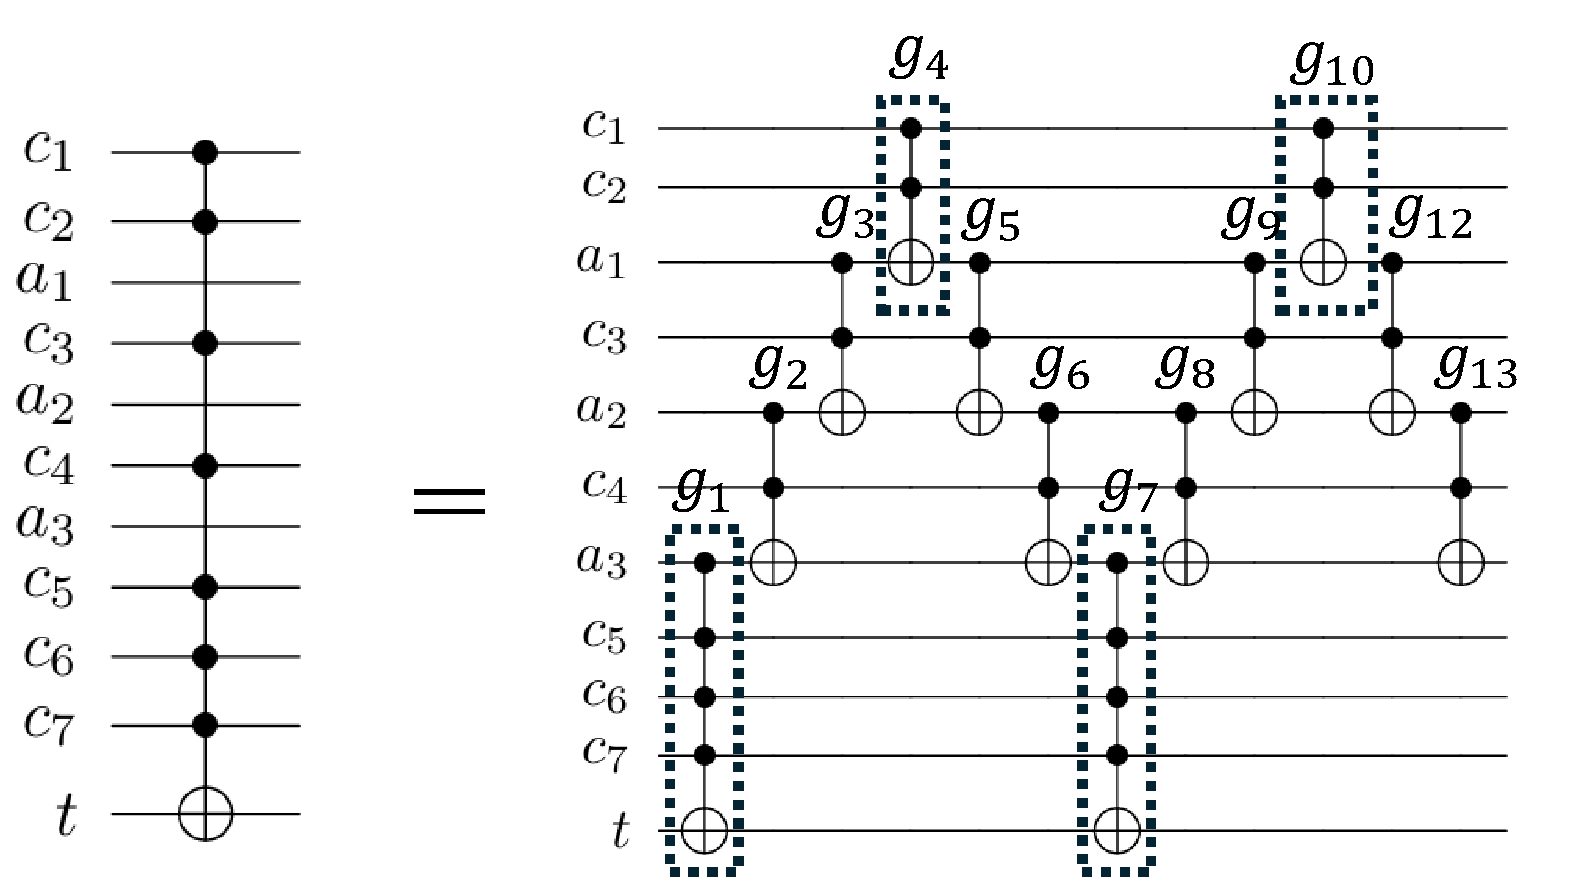
\includegraphics[width=10cm]{img/baker.pdf}
\caption{Example of application of method ~3 to MCT gate with $c=7$ and 3 undefined auxiliary bits}
\label{baker}
\end{figure}
\par
The Toffoli gate that appears when applying the decomposition of method ~3 to the MCT gate can be replaced with a $CCiZ, CCi\omega Z$ gate.
We will explain this method.
First, the Toffoli gate in Figure ~\ref{baker} can be replaced with a $CCiZ, CCiZ^{\dag}$ gate.
An example is shown in Figure ~\ref{baker_cciz}.
\begin{figure}[tbp]
\centering
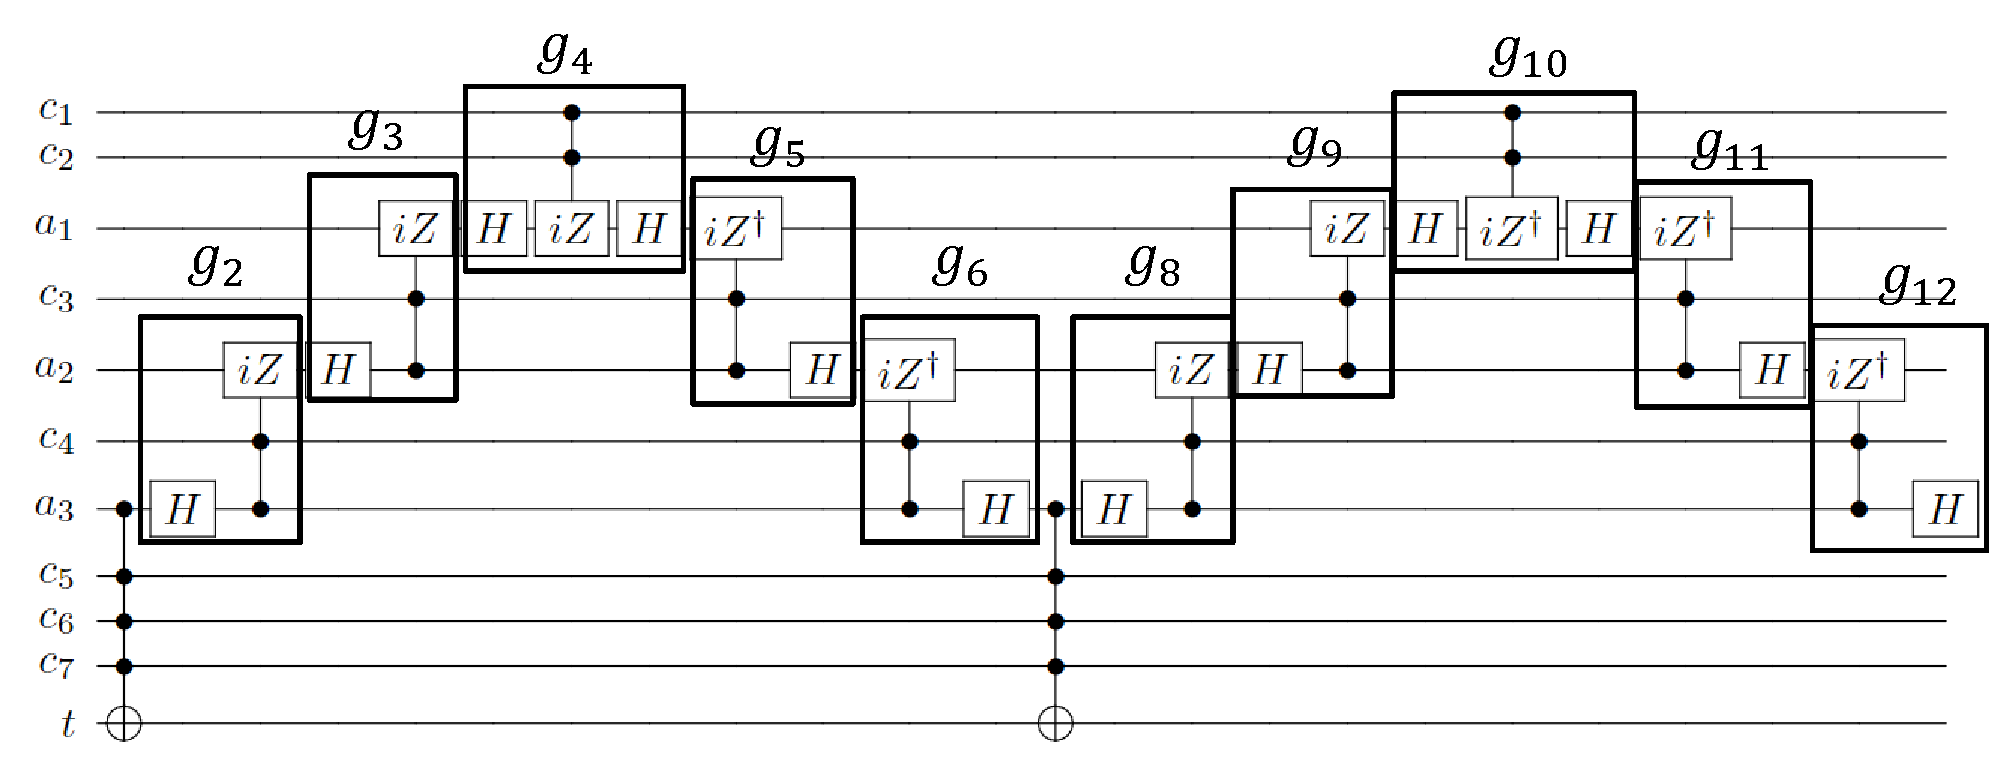
\includegraphics[width=15cm]{img/baker_izgate_transform.pdf}
\caption{Replacement of the Toffoli gate in Figure~\ref{baker} with a $CCiZ$ gate}
\label{baker_cciz}
\end{figure}
A pair of Toffoli gates with the same input and output bits is
Figure~\ref{toffoli_transform} $CCZ$ gates can be replaced with $CCiZ$ gates as shown in Figure~\ref{zgate_transform}.

As shown in Figure~\ref{zgate_to_iz},

$CCZ$ gates can be considered to be the same as the target bit and the control bit.

As shown in Figure~\ref{zgate_to_iz}, $CCZ$ gates can be replaced with $CCiZ$ gates and $CS$ gates, or $CCiZ^{\dag}$ gates and $CS^{\dag}$ gates.

The $CS$ gates and $CS^{\dag}$ gates arranged as shown in Figure~\ref{izgate_transform} cancel each other's operations.

Therefore, the same operation can be expressed even if the $CS$ gates and $CS^{\dag}$ gates are eliminated.

In this way, a pair of Toffoli gates with the same input and output can be replaced with a pair of $CCiZ, CCiZ^{\dag}$ gates.
Therefore, the Toffoli gate in Figure~\ref{baker} can be replaced with $CCiZ, CCiZ^{\dag}$ gates as shown in Figure~\ref{baker_cciz}.
\par
As shown in Figure~\ref{baker_cciomegaz},

\bout{$CCiZ, CCiZ^{\dag}$ gates in Figure~\ref{baker_cciz} can be replaced with $CCi\omega Z$ gates and $T^{\dag}$ gates,

$CCi\omega Z^{\dag}$ gates and $T$ gates, respectively. }

$T, T^{\dag}$ gates in Figure~\ref{baker_cciomegaz} can be deleted because their operations cancel each other out.
In addition, for the $T^{\dag}, T$ gates $T_{1}, T_{8}$ and $T_{2}, T_{7}$ in Figure~\ref{baker_cciomegaz}, the operation of the \bout{$T^{\dag}$} gates of $T_{1}, T_{2}$ on the left side is restored by the \bout{$T$ gates} of $T_{7}, T_{8}$ on the right side. 
These gates can also be deleted because their absence does not affect the results of the operation.
In this way, the Toffoli gates that appear in the decomposition of Method~3 can be replaced with $CCiZ, CCi\omega Z$ gates.
\begin{figure}[tbp]
\centering
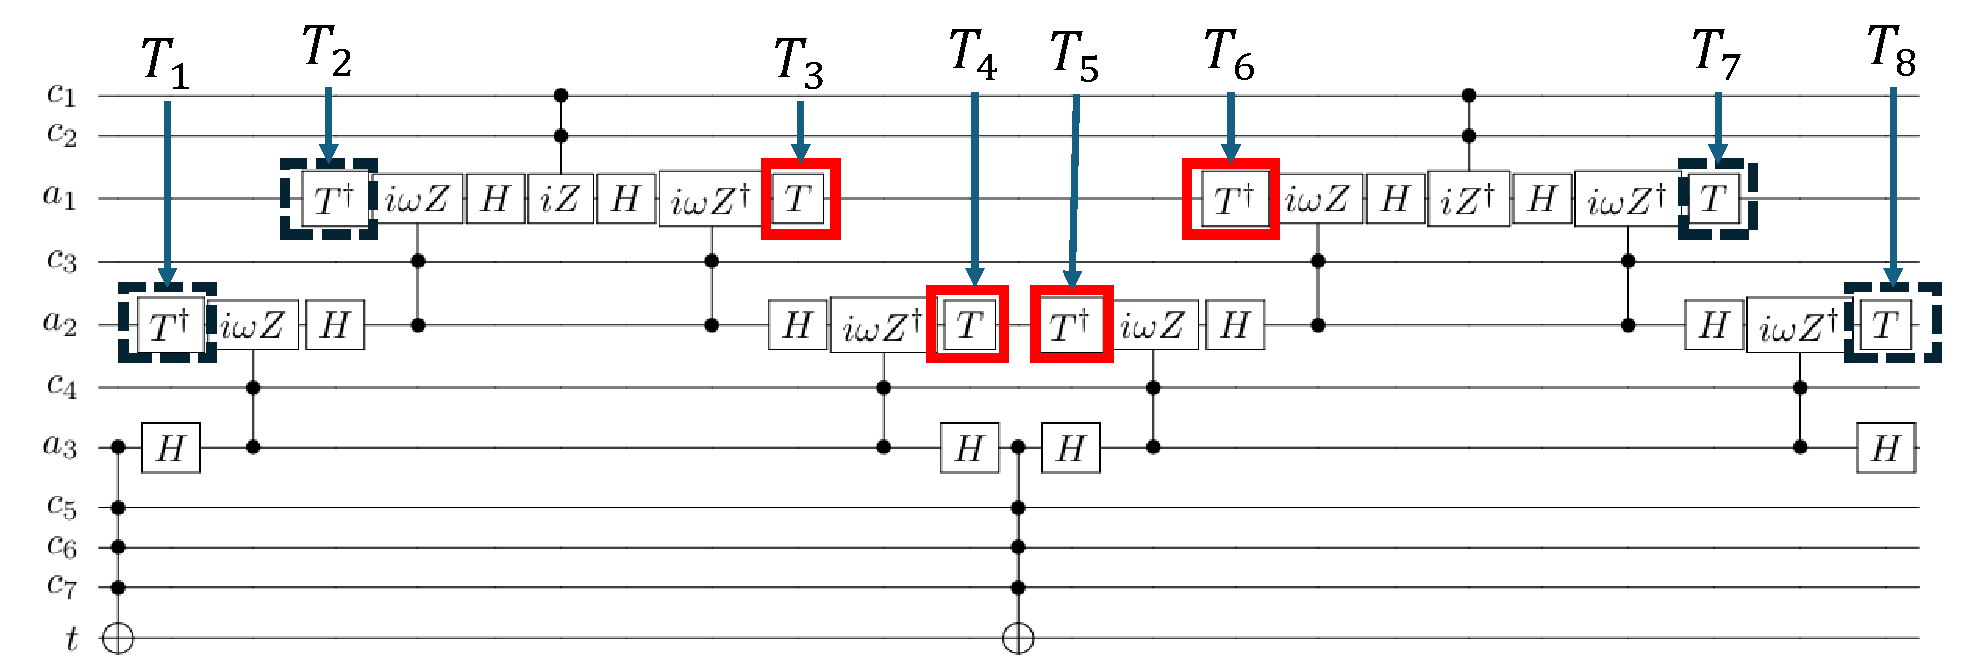
\includegraphics[width=15cm]{img/baker_iomegaz.pdf}
\caption{An example in which the \bout{$CCiZ, CCiZ^{\dag}$ gates in Figure~\ref{baker_cciz} are replaced with $CCi\omega Z, T^{\dag}$ gates and $CCi\omega Z^{\dag}, T$ gates, respectively}}
\label{baker_cciomegaz}
\end{figure}
\subsection{Method~4}
In this section,
we explain the decomposition method\cite{niemann2019t} of MCT gates using auxiliary bits whose value is 0.
From now on, this method will be called Method~4.
Method~4 decomposes MCT gates by dividing the cases into based on the number of auxiliary bits whose value is 0, $k$, used in the decomposition.
Also, let $d$ be the number of auxiliary bits with indefinite values used in the decomposition.

Let $a_{1},\dots, a_{k}$ be the $k$ auxiliary bits with a value of 0. Let $c$ be the number of control bits of the MCT gate to be decomposed.

\subsection*{In the case of $1\leq k \leq \frac{c}{2}$}

In the case of $1\leq k \leq \frac{c}{2}$,
the MCT gate to be decomposed is decomposed into three stages of MCT gates, as shown in Figure~\ref{niemann}.

Method~1 is applied to each of the decomposed MCT gates to perform the decomposition.

In Method~4, as shown in Figure~\ref{niemann},
the T-depth is reduced by arranging MCT gates in parallel in the first and third stages by the number of $k$.

\par
We will explain how to decompose MCT gates into three stages.
First, the $c$ control bits of the MCT gate to be decomposed are divided into a set of $k+1$ control bits $C_{1},\dots,C_{k+1}$.
The number of elements in this divided set of control bits is denoted as $|C_{i}|$.
The arrangement of the three-stage MCT gates is as follows.
\begin{enumerate}[First stage]
\item $C_{1},\dots,C_{k}$ are the respective control bits, and $k$ MCT gates are placed with $a_{1},\dots,a_{k}$ as their respective target bits.
\item $C_{k+1}$ and the $k$ auxiliary bits $a_{1},\dots,a_{k}$ are the control bits, and an MCT gate with the target bit $t$ of the original MCT gate as the target bit is placed in the second stage.
\item The third row contains the same $k$ MCT gates as the first row.

The third row MCT gate restores the value of the ancillary bits that are 0 to 0.

\end{enumerate}
\begin{figure}[tbp]

\centering

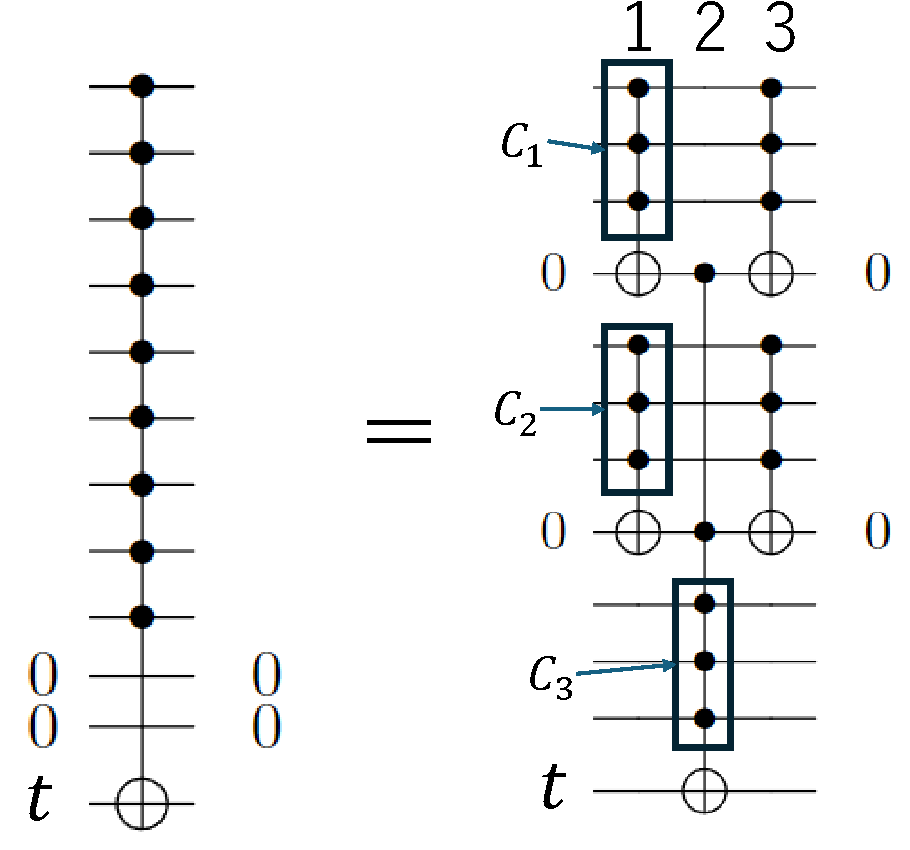
\includegraphics[width=6cm]{img/niemann.pdf}

\caption{Decomposition example of MCT gate for $c=9$ using two ancillary bits with a value of 0}

\label{niemann}

\end{figure}

\par
Method~1 is used to decompose the MCT gates arranged in three rows.

Therefore, to decompose these MCT gates,
ancillary bits with undefined values are required according to the number of control bits for each row.

The number of ancillary bits with undefined values required for each row must be considered,

and it is necessary to determine
$C_{1},\dots,C_{k+1}$.

\par
The second row MCT gate has $k+|C_{k+1}|$ control bits.
Therefore, to apply method ~1 to the second-stage MCT gate,
$k+|C_{k+1}-2|$ auxiliary bits with indefinite values are required.
Bits not used in the second-stage MCT gate can be used as auxiliary bits with indefinite values.
Therefore,
$|C_{1}|+,\dots, +|C_{k}|$ bits used as control bits in the first stage
can be used as auxiliary bits with indefinite values in the second-stage MCT gate.
To apply the decomposition of method ~1 to the second-stage MCT gate,
equation ~\ref{eq:2danme} must be satisfied.
\begin{equation}\label{eq:2danme}
d+|C_{1}|+\dots +|C_{k}|\geq (k+|C_{k+1}|)-2
\end{equation}
\par
To apply method~1 to the MCT gates in the first and third stages,
$(|C_{1}|-2)+\dots+(|C_{k}|-2)$ auxiliary bits with undefined values are required.
The bits not used in the first and third stages can be used as undefined auxiliary bits.
Therefore,
$|C_{k+1}|$ bits used as control bits in the second stage and
the target bit $t$ in the second stage can be used as undefined auxiliary bits.
In addition, considering the number $d$ of undefined auxiliary bits used in the decomposition,
equation \ref{eq:13danme} must be satisfied to apply method~1 to the MCT gates in the first and third stages.
\begin{eqnarray}\label{eq:13danme} d+|C_{k+1}|+1&\geq& (|C_{1}|-2)+\dots+(|C_{k}|-2)=|C_{1}|+\dots+|C_{k}|-2k \end{eqnarray} \par $C_{1}+\dots +C_{k+1}=c$ and From the expression~\ref{eq:2danme} and the expression~\ref{eq:13danme}, The formula ~\ref{eq:seiyaku} can be derived.
\begin{equation}\label{eq:seiyaku}
\frac{c+2-k+d}{2}\geq|C_{k+1}|\geq \frac{c-2k-d-1}{2}
\end{equation}
When decomposing MCT gates, if the value of $C_{k+1}$ is set to satisfy equation ~\ref{eq:seiyaku},
method ~1 can be applied to each decomposed MCT gate.
\par
If the MCT gates are simply decomposed to satisfy equation ~\ref{eq:seiyaku},
the overall T-depth may become large.
Therefore,
$C_{1},\dots,C_{k+1}$ must be determined so that the overall \bout{T-depth becomes small}.
The method for determining this consists of the following three steps.
\begin{enumerate}[Step (1)]
\item $|C_{k+1}|$ is the maximum value that satisfies the formula \ref{eq:seiyaku}.
Then, move the remaining $c-|C_{k+1}|$ control bits evenly to $C_{1},\dots,C_{k}$.
At this time, the difference between $|C_{1}|,\dots,|C_{k}|$ is allowed to be up to 1.
\item Move the control bits from $C_{k+1}$ to $C_{1},\dots,C_{k}$ so that the maximum number of $|C_{1}|,\dots,|C_{k}|$ does not increase.
At this time, move so that $|C_{k+1}|$ satisfies the formula \ref{eq:seiyaku}.
\item
If $k\geq 2$ and three or more control bits can be moved from $C_{k+1}$ so that equation \ref{eq:seiyaku} is satisfied,

move the control bits one by one to $C_{1},C_{2}$ and return to step (2).

If not, end.

\end{enumerate}

Based on the above procedure, $C_{1},\dots,C_{k+1}$ are determined and the MCT gates are decomposed into three stages.

\par
When decomposed using $k=\frac{c}{2}$ auxiliary bits with a value of 0,

as shown in Figure~\ref{niemann_frac_c_2},

the number of control bits for all MCT gates in the first and third stages

is 2.

In this case, the first and third stages are the optimal division of the control bits.

Therefore, even if more auxiliary bits with a value of 0 are added,

the control bits in the first and third stages cannot be further divided.
\begin{figure}[tbp]
\centering
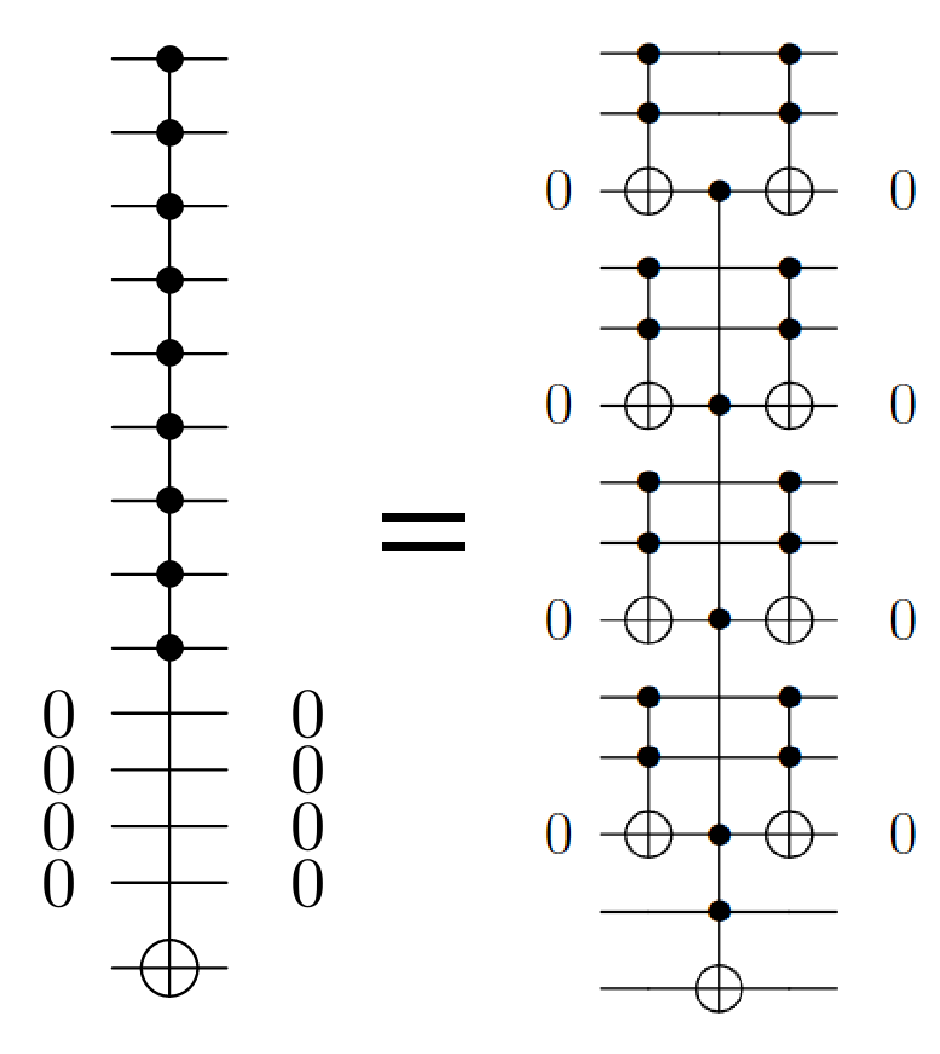
\includegraphics[width=8cm]{img/niemann_k_frac_c_2.pdf}
\caption{Example of decomposition of MCT gate $c=9$ using four auxiliary bits with a value of 0}
\label{niemann_frac_c_2}
\end{figure}
\subsection*{When $\frac{c}{2} \bout{<} k \leq c-2$}
When $k>\frac{c}{2}$,
first, use $\lfloor\frac{c}{2}\rfloor$ auxiliary bits with a value of 0 to decompose all MCT gates in the first and third stages so that the number of control bits is 2.
In this case, the number of control bits of the MCT gate in the second stage is $c'=c-\lfloor \frac{c}{2}\rfloor$.
The remaining number of auxiliary bits with a value of 0 is $k'=k-\lfloor \frac{c}{2} \rfloor$.

Using the remaining $k'$ auxiliary bits with a value of 0,
\rout{When $k'\leq \frac{c'}{2}$ and when $k' > \frac{c'}{2}$,
the MCT gate with $c'$ control bits in the second stage is decomposed. }
\par
When $k=c-2$,
as shown in Figure~\ref{niemann_c_2},
the number of control bits for all decomposed MCT gates is 2.

Therefore, even if more than $c-2$ auxiliary bits with a value of 0 are added,
the control bits cannot be further divided. 
\begin{figure}[tbp]
\centering
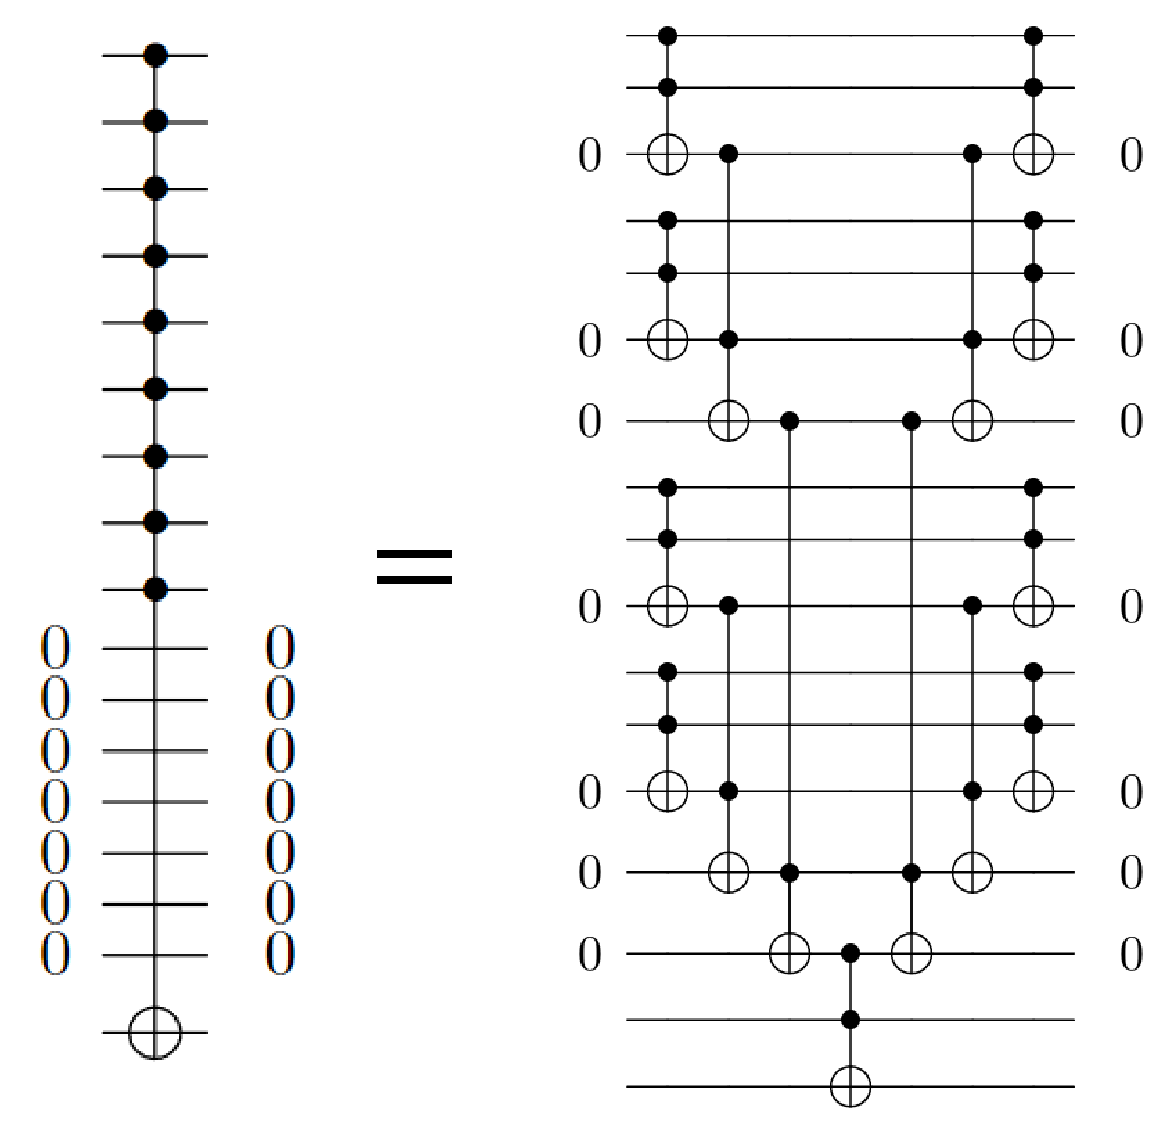
\includegraphics[width=9cm]{img/niemann_c_2.pdf}
\caption{Decomposition example of MCT gate for $c=9$ using 7 ancillary bits with value 0}
\label{niemann_c_2}
\end{figure}
